%SAVEDAT= 1453457093
\documentclass[11pt, a4paper]{article} 
\usepackage{slashed,jheppub,multirow,relsize,soul}
\usepackage[normalem]{ulem}
\usepackage{color}
\usepackage{subcaption}
\usepackage{mathabx}
\usepackage[utf8]{inputenc} 

\newcommand{\refeq}[1]{Eq.~(\ref{#1})}
\newcommand{\refeqs}[2]{Eqs.~(\ref{#1})~and~(\ref{#2})}
\newcommand{\refeqss}[3]{Eqs.~(\ref{#1}), (\ref{#2})~and~(\ref{#3})}
\newcommand{\reffig}[1]{Fig.~\ref{#1}}
\newcommand{\reffigs}[2]{Figs.~\ref{#1}~and~\ref{#2}}
\newcommand{\refsec}[1]{Section~\ref{#1}}
\newcommand{\refapp}[1]{Appendix~\ref{#1}}
\newcommand{\reftab}[1]{Table~\ref{#1}}
\newcommand{\refref}[1]{Ref.~\cite{#1}}
\newcommand{\refrefs}[2]{Refs.~\cite{#1}~and~\cite{#2}}

\def\abelian{abelian}
\def\nonabelian{non-abelian}
\def\lagrangian{lagrangian}
\def\eg{\emph{e.g.}}
\def\ie{\emph{i.e.}}
\def\aka{\emph{a.k.a.}}
\def\muboone{MicroBooNE}
\def\icarus{Icarus}
\def\minerva{MINER$\nu$A}

%%%%%%% A few editorial macros. %%%%%%%

\newcommand{\lorem}{ \textcolor[rgb]{0.8,0.8,0.8}{Lorem ipsum dolor sit amet, constetur
adipiscing elit, sed do eiusmod tempor incididunt ut labore et dolore magna
aliqua. Ut enim ad minim veniam, quis nostrud exercitation ullamco laboris nisi
ut aliquip ex ea commodo consequat. Duis aute irure dolor in reprehenderit in
voluptate velit esse cillum dolore eu fugiat nulla pariatur. Excepteur sint
occaecat cupidatat non proident, sunt in culpa qui officia deserunt mollit anim
id est laborum.}}

\newcounter{CommentCount}
\setcounter{CommentCount}{1}

\newcommand{\marcom}[2]{\textsuperscript{\textcolor{#1}{\theCommentCount}}\marginpar{\textsuperscript{\textcolor{#1}{\theCommentCount}}\textcolor{#1}{{\small#1: #2}}}\stepcounter{CommentCount}}

\newcommand{\newtext}[2]{\textcolor{#1}{\ul{#2}}}

% Add your own colour down here... 
\definecolor{PB}{rgb}{0.9,0,0}
\definecolor{MARK}{rgb}{0.612, 0.153, 0.69}

%%%%%%%%%%%%%%%%%%%%%%%%%%%%%%%%%%%%%%%


\title{Decays of MeV scale sterile neutrinos at the Fermilab Short-Baseline Neutrino complex}

\author{Peter Ballett,}
\author{Silvia Pascoli}
\author{and Mark Ross-Lonergan}

\affiliation{Institute for Particle Physics Phenomenology, Department of
Physics, Durham University, South Road, Durham DH1 3LE, United Kingdom}

\emailAdd{peter.ballett@durham.ac.uk}
\emailAdd{silvia.pascoli@durham.ac.uk}
\emailAdd{mark.ross-lonergan@durham.ac.uk}

\abstract{
%
We study the sensitivity of the Short-Baseline Neutrino (SBN) programme at
Fermilab to MeV sterile neutrino decay in both a minimal extension and more
generic beyond the Standard Model scenarios. We provide estimates for the
bounds that first $\mu$BooNE and subsequently the full SBN complex can be
expected to place on the parameter spaces of these models. We show that the
facility can in many cases extend existing bounds on $\nu_N \rightarrow
\nu_\alpha e^+ e^-$ and $\nu_N \rightarrow l^- \pi^+$ whilst, due to the strong
particle identification capabilities of liquid-Argon technology, also place
bounds on as yet unconstrained channels $\nu_N \rightarrow \gamma \nu_\alpha$
and $\nu_N \rightarrow \nu_\alpha \pi^0$.
%
We then compare the signals of decays in flight to other models with sterile
neutrinos.  We show that significant differences exist between the spectra of a
decay in flight signal and alternative models motivated by the MiniBooNE
excess.
%
We also show that the particular design of SBN, with three detectors at
different baselines, in principle allows for observable structure in the timing
distributions of events and we assess the regions of parameter space for which
such a measurement could be expected. 
%
}

\begin{document} 

\maketitle

\section{Introduction}

The neutrino sector of the Standard Model (SM) is known to be incomplete. The
observation of oscillatory behaviour between neutrino flavour states suggests a
set of mass matrices with off-diagonal terms in the flavour basis. There are
many ways that have been suggested in the literature to explain neutrino masses
from a theoretical perspective, ranging from the popular see-saw scenarios
\cite{Minkowski:1977sc, GellMann:1980vs, Mohapatra:1979ia} to radiative mass
generation \cite{XXX} or even more involved constructions \cite{XXX}. It will
ultimately be the role of phenomenology to find ways to distinguish between
candidate models, and see what can be learnt from the completion of the
neutrino sector about the structure of BSM physics.
%
However, not all models of neutrino masses lend themselves to experimental
searches. For example, the canonical Type-I see-saw \cite{Minkowski:1977sc,
GellMann:1980vs, Mohapatra:1979ia} suggests the existence of new particles with
masses around $10^{12}$--$10^{15}$ GeV, well out of reach of modern
experimental techniques.  One observable feature of some models is the presence
of novel fermionic singlets of the SM gauge group, which we shall refer to as
sterile neutrinos.  These will generically mix with the `active' neutrinos of
the SM and could alter neutrino phenomenology at observable scales. 
%
A well known example of such an effect is the short-baseline disappearance
signature associated with a sterile neutrino with a mass around the eV scale
(see \eg\ \refref{Gariazzo:2015rra} for a recent review). Such a state would
produce oscillatory effects over short distances and has been invoked to solve
the anomalies found at some short-baseline oscillation experiments.  Explaining
all anomalies in an economical fashion appears challenging in these models
\cite{Kopp:2013vaa}, but more data would be needed before a decision can be
made as to their role in the neutrino sector.

In this article, we study a complementary paradigm to the oscillatory sterile
neutrino models where sterile neutrinos exist, are produced in neutrino beams
via meson decay, but have masses sufficiently large to prevent oscillatory
effects with the active neutrinos through loss of coherence (see \eg\
\refref{Akhmedov:2009rb}).  Due to the presence of mixing effects, these
particles are not generically expected to be stable and their subsequent decays
have been enumerated \cite{Atre:2009rg} and searched for in many previous
experiments.
%
Our focus will be on estimating the potential sensitivity of the Fermilab SBN
programme \cite{Antonello:2015lea} for the search for sterile neutrinos of this
type. 
%
This experimental facility comprises of three separate detectors placed in the
Booster Neutrino Beam (BNB) at different (short) baseline distances: SBND
(previously known as LAr1-ND) at 110~m from the target, \muboone\ at 470~m and
ICARUS at 600~m.  All three detectors employ Liquid Argon (LAr) technology
giving unprecedented reconstruction and particle identification capabilities
allowing for significantly lower backgrounds than predecessor technologies. We
will focus in particular on $\mu$BooNE as it the experiment has already began
to collect data and will be first of the SBN detectors to be able to perform
such a search.
%
%\newtext{PB}{In addition to events arising from the BNB, the detectors of the
%SBN complex will also collect events associated with the NuMI beam, currently
%being used in the NO$\nu$A, MINER$\nu$A and MINOS+ experiments. This beam is
%off-axis with respect to the SBN detectors leading to significant kinematic
%differences.}
%
The SBN facility has a number of interesting features relevant to the search
for sterile neutrino decay:

\begin{enumerate}

\item The reconstruction, timing resolution and particle ID capabilities of LAr technology means
the SBN program provides an ideal scenario to study the decay in flight of
sterile neutrinos, a job which has traditionally been left for low-mass
detectors with corresponding low beam-related backgrounds. 
%
We will discuss how a very high level of background suppression can be obtained
through a simple cut-based analysis motivated by the kinematic properties
of a beam-based decay-in-flight signal. 

\item The three detectors allow for timing-based effects between 
the three detectors if the excess comes from a sterile neutrino decay 
model. As we will discuss in \refsec{sec:timing}, this means that a decaying 
sterile neutrino would have a very distinctive pattern of excess events at
SBN, unobservable to a facility with a single detector.

\item The excellent particle identification will allow for the investigation of
channels for which there are no published searches, only inferred bounds based
on minimal theoretical models. We will discuss extended models of sterile decay
where the minimal model correlations between decay channels do not hold. This
means that there are no published bounds on some channels, and a decay rate in
a traditionally excluded region could be observed at the SBN complex. In the
absence of signal, the facility could of course place the first bounds on these
signatures of new physics.

\end{enumerate} 

\begin{table}[t!]
\centering
\begin{tabular}{| l || l | l | l | l |}
	\hline
	& PS-191 & SBND & $\mu$BooNE & ICARUS \\ \hline \hline
	POT	& $0.86 \times 10^{19}$	& $6.6 \times 10^{20}$	&	$13.2 \times 10^{20}$     &  $6.6 \times 10^{20}$ \\ \hline
	Volume	& $216\text{m}^3$	&	$80\text{m}^3$	&	$62\text{m}^3$	     &   $340\text{m}^3$	\\ \hline
	$\text{Baseline}^{-2}$	& $(128 	\text{m} )^{-2}$	&$(110 \text{m} )^{-2}$	&	$(470 \text{m} )^{-2}$			     & $(600 \text{m} )^{-2}$	  \\ \hline
Ratio/PS-191 & - 	& 38.5 	& 3.3	& 5.5\\ \hline
\end{tabular}

\caption{\label{tab:exposure} A comparison of the exposure at each SBN detector compared to PS-191. One would expect all  three SBN detectors to see larger numbers of events than PS-191, while SBND sees the largest enhancement of a factor of $38.5$.}

\end{table}

Decaying heavy sterile neutrinos have been searched for at many experiments
since the early 1970s \cite{}. In the mass range of interest for SBN, the
strongest bounds on sterile which mix with electron and muon neutrinos come
from PS-191 \cite{Bernardi:1985ny}, which ran at CERN from 1983 to 1985. 
%
PS-191 was located 128m downstream of the target and $2.3^\circ$ (40 mrads) off
axis, obtained $0.86 \times 10^{19}$ POT over the course of its run-time, and
had a total detector volume of $6\times3\times12 = 216 \text{m}^3$. We can
estimate the sensitivity of the three SBN detectors and how they will compare
to PS-191 by estimating the experiments' \emph{exposure}, defined here as POT
$\times$ Vol $\times$ $R^{-2}$. We compare the three facilities to PS-191 in
\reftab{tab:exposure}, which shows that all detectors of the SBN complex expect
a larger exposure, with SBND seeing the largest enhancement by a factor of
around $40$. Although the majority of the sensitivity of the full SBN data set
will come from SBND with its larger event rates, the data will be collected at
different times --- $\mu$BooNE has already begun to take data and will be able
to search for such decays many years before SBND and ICARUS come online --- for
this reason, we will consider all detector sites in our analysis.

In addition to the larger exposure, there is also an enhancement of the
expected decay events at SBN due to its lower beam energy. The steriles at SBN
are produced by the 8 GeV BNB beam and have a softer spectrum than those
produced by the 19.2 GeV proton synchrotron beam used at PS-191. As we will
discuss in more detail in \refsec{Decays}, the probability of sterile neutrino
decay scales as $1/E_\nu$, and we would therefore expect the SBN facilities to
see more events than PS-191 for equivalent exposures.

Despite the advantage of scale at SBN, backgrounds could limit the improvement
in performance when compared to PS-191. PS-191 was purposefully built to search
for decays in flight of heavy fermions, and to minimize the background induced
by active neutrino scattering, the total mass of the detector was chosen to be
small (approximately $20$ ton)\marcom{PB}{I'm not sure I get this: do we mean
cosmics? Why wouldn't the backgrounds and signal scale in the same way?}. The
SBN detectors, whose primary goal is to study neutrino scattering, have
significantly larger masses ($112$, $66.6$ and $476$ tons respectively). We
therefore expect SBN to not only see a greater number of decay events than
PS-191, but to also see a greater background. 
%
To understand the sensitivity of SBN to heavy sterile decay, the background
rejection capabilities of LAr must be sufficiently well understood.  We will
discuss this in more detail in \refapp{sec:bg}.

\section{Sterile neutrino decay}

The most general renormalizable \lagrangian\ extending the SM to include a
single novel gauge-singlet fermion $N$ is given by
%
\begin{align}   \mathcal{L} = \mathcal{L}_\text{SM} +
\overline{N}i\slashed{\partial}N+ \frac{\mu}{2} \overline{N^\text{c}}N  +
y_\alpha\overline{L}_\alpha\tilde{H} N + y_\alpha^*
\overline{N}\widetilde{H}^*L_\alpha\label{eq:minimallag} \end{align}
%
where $y_\alpha$ denote Yukawa couplings and $\mu$ a Majorana mass term for
$N$. The extension to multiple new fermions involves promoting $y$ and $\mu$ to
matrices with indices for the new states, but will offer no real
phenomenological difference in the current work.\footnote{The minimal single
$N$ extension does not allow for the observed masses of the neutrinos, as the
mass matrix is rank 1. We assume that an appropriate extension has been
introduced to satisfy neutrino oscillation data while introducing no new
dynamics at the lower energy scales of interest.} Much work has been done
understanding the phenomenology of novel neutral states, which varies
significantly over their large parameter spaces. 
%
If these particles have masses around $10^{15}$ GeV they could provide a
natural way to suppress the size of active neutrino masses through the Type I
or III see-saw mechanisms \cite{Minkowski:1977sc, GellMann:1980vs,
Mohapatra:1979ia}. A lighter neutral fermion, with a mass around the keV scale,
remains a promising dark matter candidate \cite{Adhikari:2016bei}. A synthesis
of these ideas is found in the so-called $\nu$MSM which simultaneously can
explain dark matter, neutrino masses and successful baryogenesis
\cite{Asaka:2005pn}. 
%
If the sterile gets lighter still, with masses at the eV scale or below, an
important observable effects might exist in neutrino oscillation experiments.
Indeed, eV scale particles have been proposed to alleviate short-baseline
oscillation anomalies; although, no minimal solution seems to provide a
compelling universal improvement to the current data \cite{Kopp:2013vaa}. 
%

For steriles which are light enough to be produced in a neutrino beam,
typically with masses below the $D$-meson mass scale $m_{\nu_N} \lesssim
2$~GeV, there is a qualitative divide in the phenomenology somewhere between
keV and eV energies\footnote{The precise mass range depends on details of the
process under consideration.}. If the sterile neutrinos are massive enough for
their mass-splittings between the light neutrinos to be larger than the
wavepacket uncertainty associated with the production mechanism, they no longer
oscillate \cite{Akhmedov:2009rb}.  
%
Once oscillation is suppressed, neutral particles produced in the beam will
propagate towards the detector and may be observed by their subsequent decay
into SM particles. Experiments seeking to measure such decays are generally
known as beam dump experiments where proton collisions with a target produce
particles to be observed down-wind of the source \cite{CooperSarkar:1985nh,
Bergsma:1985is, Vaitaitis:1999wq, Bernardi:1985ny, Bernardi:1987ek,
Anelli:2015pba, Alekhin:2015byh}. It has been pointed out that the difference
between a beam dump and a conventional neutrino beam is more a matter of
philosophy, and we can expect many experiments to have some sensitivity to
novel heavy states \cite{Gorbunov:2007ak, Asaka:2012bb, Adams:2013qkq}. 
%
For the BNB, we can estimate the mass at which this decoupling occurs as
follows: the decay pipe for BNB is around $50$~m in length, which is
considerably shorter than the decay lengths of the mesons in the beam.
Therefore this length defines the wavepacket width at production.  The relevant
parameter is the decoherence parameter \cite{Akhmedov:2009rb, Hernandez:2011rs}
%
\[  \xi = 2\pi \frac{\lambda_\text{d}}{\lambda_\nu}, \]
%
where $\lambda_\text{d} = 50$~m and $\lambda_\nu$ is the standard neutrino
oscillation length $\lambda_\nu = \Delta m^2/4E_\nu$. For $\xi\gg1$ the wave
packet is insufficiently broad to accommodate a coherence superposition of the
heavy and light neutrino states. We estimate that this occurs at 
%
\[  \Delta m^2 \gtrsim 20~\text{eV}^2. \] 
%
In this article we study the region of MeV scale sterile masses. These are
heavy enough to forbid oscillatory effects while light enough to be have
significant production from the meson decays associated with a conventional
neutrino beam. 

The observable signature in this model is the direct decay of the new fermion
into SM particles. In the minimal \lagrangian\ in \refeq{eq:minimallag}, the
only direct couplings to new sterile fermions are neutrino Higgs interactions.
However, these couplings generate off-diagonal neutrino bilinears below the
electroweak symmetry breaking scale, which leads to mass mixing between the
$4+$ flavours of neutrinos. This generates production and decay mechanisms of
many kinds for the state $N$ through mass insertion on an active neutrino
fermion line in a gauge mediated process. These decays have been studied
extensively in the literature \cite{Atre:2009rg} and depend only on the size of
neutrino mixing to various flavours, parameterized by the elements of an
extended $4\times4$ PMNS matrix,
%
\[ U_{e4}, \qquad U_{\mu 4} \qquad \text{and} \qquad U_{\tau 4},  \]
%
and the mass of the state $N$ itself. The branching ratios for these decays are
shown in \reffig{fig:branchingratios} as a function of mass for the case if the
new state mixes with all flavours of active neutrino equally $U_{e4}=U_{\mu
4}=U_{\tau 4}$. The main effect of the flavour structure is to
forbid certain decays which require certain elements of the mixing matrix. This, in turn, affects the possible production
mechanisms for these particles. In a conventional neutrino beam, most neutrinos
are derived from meson decay (or secondary $\mu^\pm$ decays). If $U_{e4}=U_{\mu
4}=0$, such decays with a mass insertion for the sterile neutrino are
impossible for pions or kaons.For this reason, we will mainly focus on mixing with the first two generations. This parameter space will be probed by working
at higher energies, where the neutral fermions can be produced by decays of
charmed mesons such as $D^\pm$, by the SHiPS experiment \cite{Alekhin:2015byh, Anelli:2015pba}.   

We focus on five decays in our study, which have the largest branching ratios
of all channels with visible decay products over the mass range producable from pion and kaon decay, $m_{\nu_N} \lesssim m_K$.

\begin{align*}
	\pi^\pm / K^\pm \longrightarrow \overbrace{l^\pm \nu_N}^{\text{via } U_{e4} \text{ or } U_{\mu 4}}  &\longrightarrow  l^\pm \pi^\mp, \\
						& \drsh \nu_\alpha e^+ e^-, \\
						& \drsh \nu_\alpha \gamma, \\
						& \drsh \nu_\alpha \pi^0. \\
\end{align*}


\begin{figure}[t]
%
\centering
%
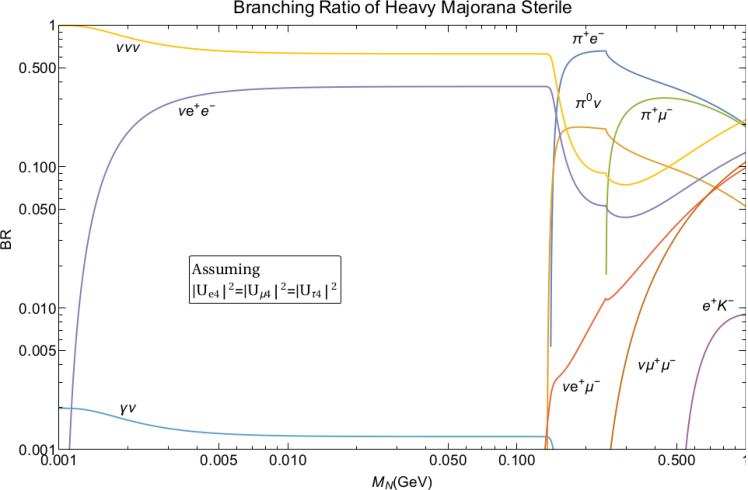
\includegraphics[width=0.8\textwidth]{figures/bounds1.pdf}
%
%
\caption{\label{fig:branchingratios}The branching ratios for sterile neutrino
decays in the minimal 3 sterile SM extension, with masses between 1 MeV and 0.5
GeV. Heavier steriles will not be produced in great numbers in the BNB beam due
to the very small componant of heavier mesons in the secondary beam. This plot
assumes equal mixing with all active flavours. Note that below 100 MeV, $\nu_N
\rightarrow \nu_\alpha e^+ e^-$ is by far the most dominant visible decay.}
%
\end{figure}

\subsection{Minimal model}

We define the minimal sterile neutrino model by the Lagrangian in
\refeq{eq:minimallag}. This corresponds to the best known model of sterile
neutrino phenomenology: the UV-complete Type I see-saw. Decays of sterile
neutrinos in such a model have been studied in \refref{}, and we briefly
summarize the important results.

For sterile neutrino masses less than the pion mass, the dominant visible decay
will be into an electron-positron pair as can be seen from
\reffig{fig:branchingratios}. This is true regardless of the flavour structure
of the mixing matrix. The decay rate for this channel is given by 
%
\[ \Gamma\left(\nu_N\to \nu_i e^+e^-\right) =
\frac{G_\text{F}^2m_N^5}{96\pi^3}I_1\left(0,\frac{m_e}{m_N},\frac{ m_e}{m_N}\right).  \]
%
where 
\begin{align}
	I_1(x,y,z) & =12 \int_{(x+y)^2}^{(1-z)^2} \frac{ds}{s}(s-x^2-y^2)(1+z^2-s)\sqrt{\lambda(s,x^2,y^2)}\sqrt{\lambda(1,s,z^2)},\\
\lambda(a,b,c) &= a^2+b^2+c^2 - 2ab-2bc-2ca.
\end{align}

%
Decays of this type would generally fall into two categories of events at a LAr
detector, and accordingly we divide our analysis. The first event sample will
attempt to measure events where two tracks are resolved and two
electron-induced electromagnetic showers are observed.
%
The second sample consists of events for which the identification of two
electron-like showers is impossible. In this case, the signal would be identical
to a single photon pair-conversion. We expect a larger background for this
scenario, but as we will show, we get sizable event numbers in this channel due
to the sterile neutrino's high energy, and a tight cut on the angular
distribution can make it sensitive to sterile decays.

Also possible at these low masses, the radiative decay
$\nu_N\to\nu_i\gamma$ would generate an interesting single photon
signal \cite{PhysRevD.25.766}. In the minimal model the decay rate goes as
%
\[ \Gamma(\nu_N\to\nu_i\gamma) = \frac{G_\text{F}^2m_N^5 |U_{\alpha 4}|^2}{192 \pi^3} \left( \frac{27 \alpha}{32 \pi} \right), \]
%
this decay channel will be very smal and the total decay rate can be estimated
at around $\Gamma(\nu_N\to\nu_i\gamma)/(\text{GeV}) \approx 10^{-20}
(m_N/\text{GeV})^5$.  

When the mass of the sterile neutrino is greater than the kinematic threshold
for the production of a neutral pion, a new decay dominates $\nu_N\to\nu_i
\pi^0$. The decay rate for this process is given by
%
\[ \Gamma\left(\nu_N \to \nu_i \pi^0\right) =
\frac{G_\text{F}^2f_\pi^2m_N^3}{64\pi} \left[1-\left( \frac{m_\pi}{m_N}
\right)^2\right].  \]

The next channel appears at the kinematic threshold for charged pion production
with a charged lepton. If mixing between the heavy mass state and the electron
neutrino is present, this decay occurs almost immediately after the $\nu\pi^0$
channel opens. However, if this mixing is negligible, there is a gap the size of
the muon mass before the $\mu^\pm\pi^\mp$ channel opens. As can be seen from
\reffig{fig:branchingratios}, these decays dominate the visible decays when
they are allowed. These decays have a similar scaling behaviour of the decay
rate to the $\nu\pi^0$ channel with an equivalent dependence on the pion
structure constant,
%
\[ \Gamma\left(\nu_N \to l^\pm\pi^\mp\right) =
	\left|U_{l4}\right|^2\frac{G_\text{F}^2f_\pi^2 |V_{ud}|^2  m_N^3}{16\pi}I\left(\frac{m_l^2}{m_\pi^2} , \frac{m_N^2}{m_\pi^2}\right) ,
\]
with 
\[
	I(x,y) = \left[ \left( 1+x+y\right) \left(1+x\right) -4 x\right] \lambda^\frac{1}{2}\left(1,x,y\right)
\]

As can be seen from \reffig{fig:branchingratios} there are several additional
decays possible $\nu_N \rightarrow \nu_\alpha \mu^+ \mu^-$ and $\nu_N
\rightarrow \nu_\alpha e^+ \mu^-$, however, in the kinematic region allowed
under the assumption the steriles were produced in pion and kaon decays these
channels have sub dominant branching ratios and are not included in this
analysis.

\subsection{Non-minimal models}

An important feature of the minimal model that we have discussed so far is the
all or nothing approach to decay rates: all decay processes of the sterile
neutrino are weak processes scaled by a mixing matrix element. 
%
Therefore it is the three mixing matrix elements $U_{\alpha 4}$ which dictate
the magnitude of all the decay rates. This is a great asset when trying to
constrain the  minimal model, for example it allows us to convert any
non-observation of a signal into a bound on the mixing matrix, and allows us to
reinterpret bounds on any one decay rate onto the expected decay rates for
other channels, such as $\nu_N \rightarrow \nu_\alpha e^+ e^-$ non-observation
being used to bound $\nu_N \rightarrow \nu_\alpha \pi^0$ despite no experiment
to-date reporting the results of such a search. 
%
However, this asset becomes a bias when used in a general search for novel
neutral states. Although such low-scale see-saws are a viable region of
parameter space, they lack a theoretically appealing mechanism to explain the
sub-electroweak sterile neutrino mass scale nor the sizes of neutrino masses.
Although alternative models exist which can provide a light neutral particle
and a mechanism to generate light neutrino masses, they rely on extended field
content or interactions.
%
Indeed it has been stressed before that a light sterile neutrino would be a
sign of some non-trivial new physics \cite{delAguila:2008ir}. To exploit the
most general constraints on the low-energy approximation to the full theory we
use effective field theory. The effective field theory of a SM extension
involving new sterile fermions has been presented at dimension 5
\cite{delAguila:2008ir,Aparici:2009fh}, dimension 6 \cite{delAguila:2008ir} and
dimension 7 \cite{Bhattacharya:2015vja}.
%
In \refref{Aparici:2009fh} the phenomenology of the effective operators at
dimension 5 are considered in detail. Along with the Weinberg operator, which
could be the source of a light neutrino Majorana mass term
\cite{Weinberg:1979sa}, the authors find two effective operators: an operator
coupling the sterile neutrino to the Higgs doublet and a tensorial coupling
between the sterile neutrino and the hypercharge field strength 
%
\[ \mathcal{L}_5 \supset \frac{c_1}{\Lambda}\overline{N^c}N(H^\dagger H) +
\frac{c_2}{\Lambda}\overline{N^c}\sigma^{\mu\nu}NB_{\mu\nu}. \] 
%
At energies below the electroweak scale, and after diagonalisation into mass
eigenstates for the neutrinos, these operators generate novel couplings, for
example a vertex allowing $N\to h \nu$ ($N_1\to h N_2$) or $N\to \nu Z$
($N_1\to Z N_2$) at a rate governed by the scale of new physics suppressing
these operators. See also \refref{Duarte:2016miz} for a discussion of decay
rates in the effective sterile neutrino extension up to dimension 6.

\newtext{PB}{Some comment on Gninenko:} $N\to \nu \gamma$: However, in a
non-minimal model this decay rate could be enhanced. For example, such an
enhancement has been proposed to resolve the MiniBooNE anomaly
\cite{Gninenko:2009ks,Gninenko:2010pr}. 



Although effective models of sterile neutrino decay can describe the low-scale
effects of high-scale physics, their predictions are invalid if unidentified
light degrees of freedom exist in the model. For example, models with sterile
neutrinos that also feature novel interactions can have significantly different
decay rates and branching fractions, strengthening some bounds and invalidating
others \cite{Batell:2016zod,Ballett:2016xxx}.
%
As an example, a model with a leptophilic $Z^\prime$ \cite{Foot:1994vd} could
enhance purely leptonic decay rates, such as $N\to \nu e^+\mu^-$, while not
enhancing semileptonic processes like $N\to e^\pm \pi^\mp$.  \marcom{PB}{Check
this reference. It is $\mu$-$\tau$, does what I say make sense?}


There are two points that are worth making about non-minimal models of sterile
decay.  Firstly, for any one channel, reporting the results of the
non-observation of certain decay products in terms of a mixing matrix element
is mostly harmless. We can always see this as an effective quantity
representing the rate of suppression compared to the minimal model with order 1
mixing terms. Therefore, no existing conclusions are altered. However,
correlations between channels must be given up: we can no longer assume that
the effective mixing angle for one channel is equal to the effective mixing
angle of another. This means that some channels are much more poorly
constrained than it might seem from the published bounds. For example, to the
best of our knowledge, no beam dump experiment to-date has placed bounds on
$N\to \nu\gamma$ or $N\to\nu\pi^0$; indeed, although the former channel has
bounds from tests of neutrino electromagnetic properties, the latter is bounded
to a fair weaker degree. 

Secondly, in any extended model the minimal couplings are still present. This
is an unavoidable consequence of mass-mixing between the active and sterile
sectors and the interactions of the SM. Therefore, without suspicious
cancellations (or destructive interference) between the mixing-derived and
higher-dimensional contributions to a decay, the non-observation of a signal in
a given decay channel can still be used to bound the mixing matrix element, and
therefore the minimally-correlated bounds \emph{do} apply to the Standard Model
+ mixing decay processes. 

For the reasons discussed so far, we believe it is relevant to place bounds on
the possible decays of a neutral fermion in an extended scheme which allows for
arbitrary decay rates to visible particles (within the bounds of perturbativity
and other conventional model building constraints).
%
We will focus here on the posibility for enlarged neutral current decay rates
of the mostly-sterile fermion. In this scenario, the production of the sterile
state will be largely unaffected by the new physics: heavy states will be
produced in the beam from meson decay as usual. However, we allow for an
increased rate of decay for the two channels $\Gamma_{\gamma\nu}$ and
$\Gamma_{\pi^0\nu}$.
%
When considering these enlarged decay rates, we must be careful with existing
bounds on the model, as an enlarged decay rate would affect all prior beam dump
experiments in the same way until the point where baseline dependence becomes
significant.

\newtext{MARK}{Going to add how to scale prexisting/our bounds for when you have an alpha enhancement.}

\section{\label{sec:timing}Role of event timing}


\begin{figure}[t]
%
\center
%
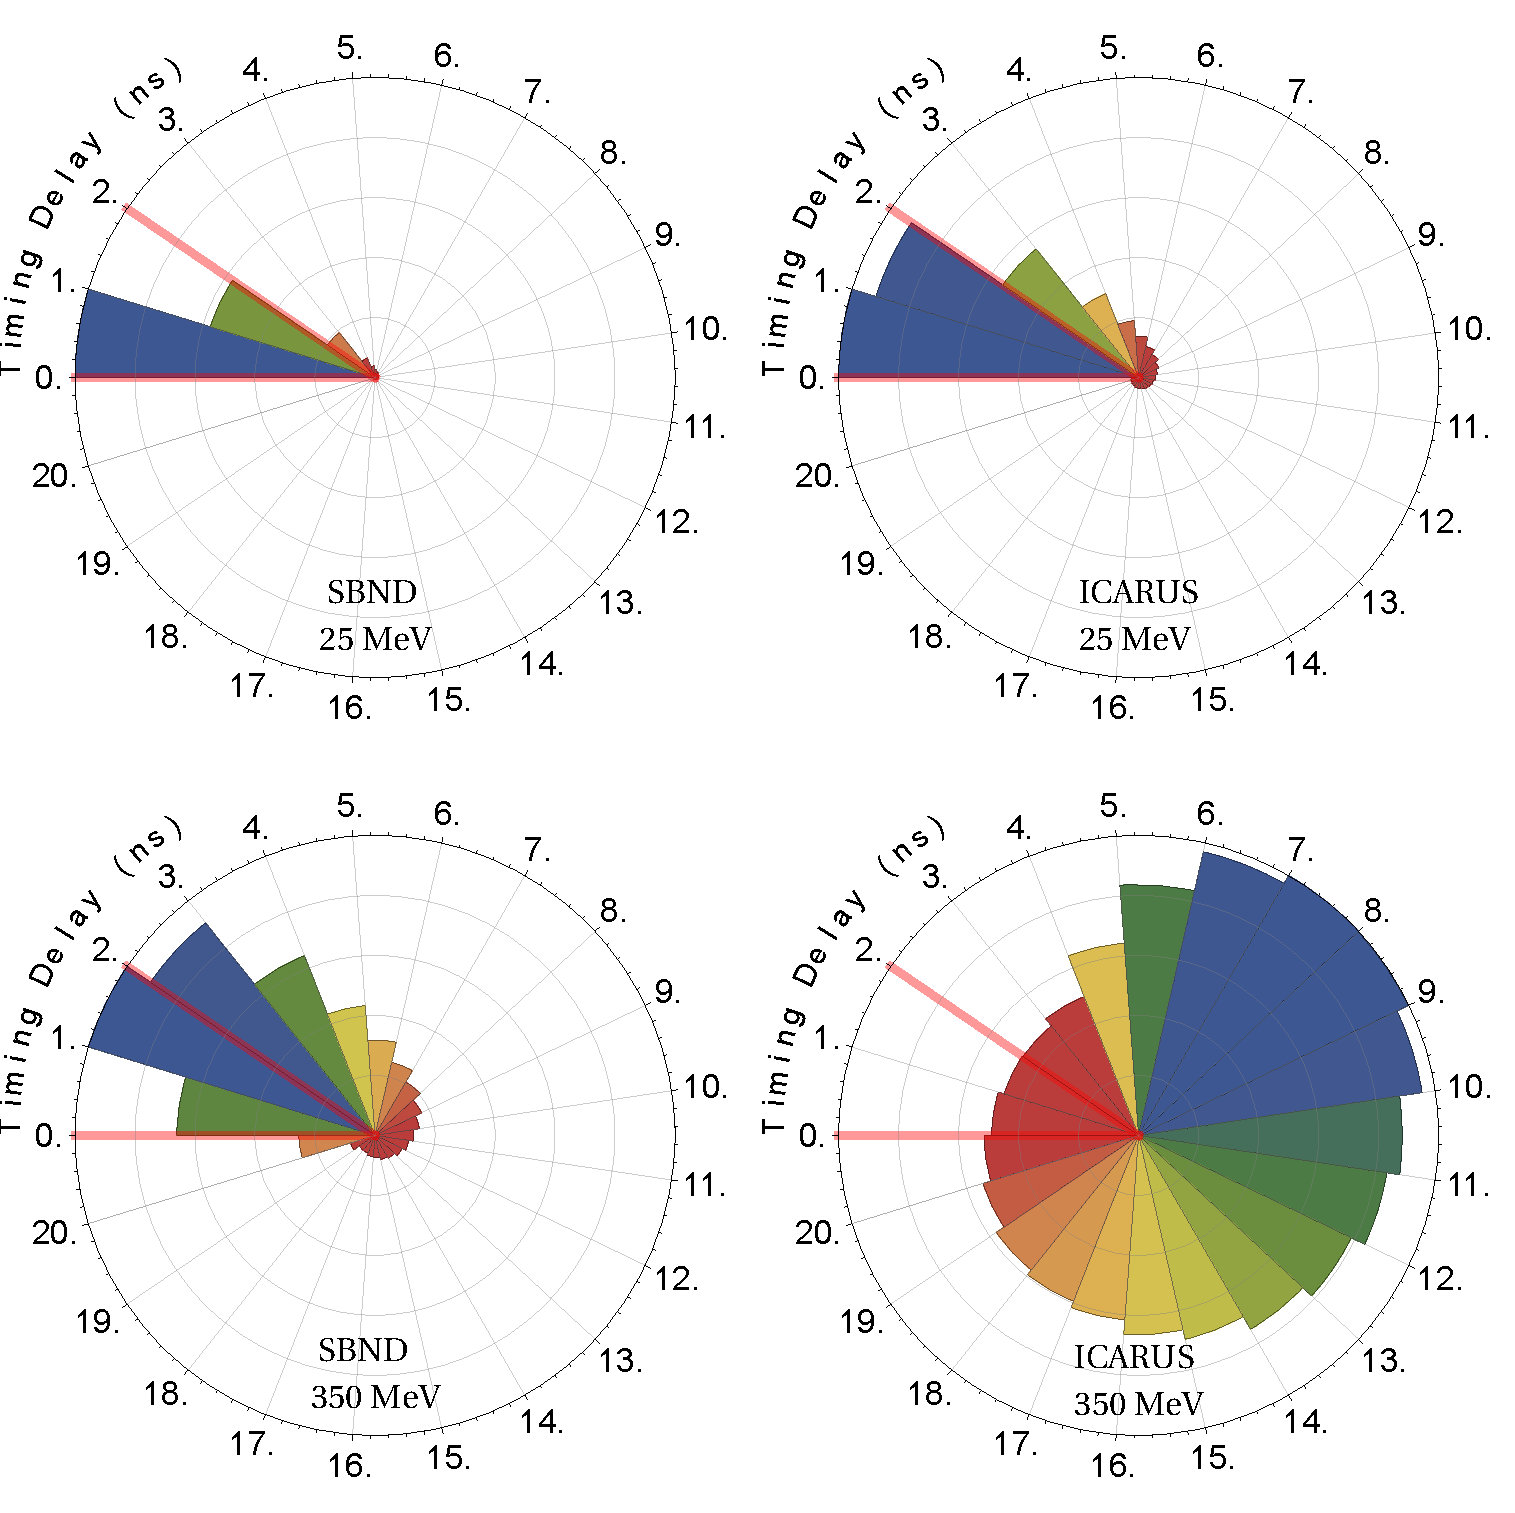
\includegraphics[width=0.75\textwidth]{figures/timing.pdf}
%
\caption{\label{fig:timing} Shown above is the timing delay of sterile neutrino
decays in nano-seconds for both a 25 MeV (top) and 350 MeV (bottom) sterile
neutrino at the SBND and and \icarus\ detectors (110 and 600m
respectively). The 2 ns beam bucket window is shown highlighted in red from 0
to 2 ns, followed by an additional 19 ns gap. The timings are calculated as a
difference to the time of flight of a active neutrino, assuming the decay
occurred in a uniform sample across the 50m BNB decay pipe. A timing resolution
of 1 ns is assumed to smear the observed events. }
%
\end{figure}

One of the interesting features of the SBN complex is the interplay of the
three detectors, operating similar technology but situated at different
baseline distances. Light neutrinos propagate and reach the furthest detector of the SBN complex after around 2
$\mu$s. In the conventional physics programme of the SBN, the timing of these events play an important
role in the analysis of backgrounds, tight timing windows are placed around the
19.2$\mu$s beam spill to limit constant rate backgrounds such as cosmogenic events.i 
Both SBND and ICARUS, however, are expected to be able to achieve significantly better timing resolution $\mathcal{O}$(1 ns), which allows for the use of both bucket and spill structure in the background analysis. The
BNB consists of 81 Radio-Frequency buckets of approximately 2ns length,
separated by 19 ns, to form the 19.2$\mu$s spill with a frequency of 3Hz
\cite{Antonello:2015ea}. Nano-second resolution allows for events in individual buckets to be identified. \muboone is omitted from this analysis as the achievable timing resolution is worse, $\approx 10$ns.

As particles with finite rest mass, these heavy neutral leptons will propagate at subluminal speeds and for larger masses can produce observable timing delays. This effect begins to become relavent when the sterile neutrinos are of MeV-scale masses and above. As the flux of decaying sterile is inversely proportional to energy, we expect many of these low energy steriles to be traveling at significantly slower speeds than their light counterparts. Shown in \reffig{fig:timing_line} below is the fraction of events that are expected to fall outside the 4ns bucket window in both SBND and ICARUS, with detailed timing spectrums of a 25 and 350 MeV sterile shown in \ref{fig:timing}.

For the lighter sterile masses around $25$ MeV, a significant fraction of decay events will end up in the beam timing window, defined to be 1ns surrounding the 2ns bucket, and must be analysed as a signal on top of the beam-related backgrounds in the standard analysis. At $m_{N}=350$ MeV, we see that while many events still fall in the in beam timing window,
both detectors see significant deviation from this with a large fraction of events populating
the inter-RF-bucket spacing where one would expect to see extremely reduced
beam-correlated backgrounds. \\
\begin{figure}[t]
%
\center
%
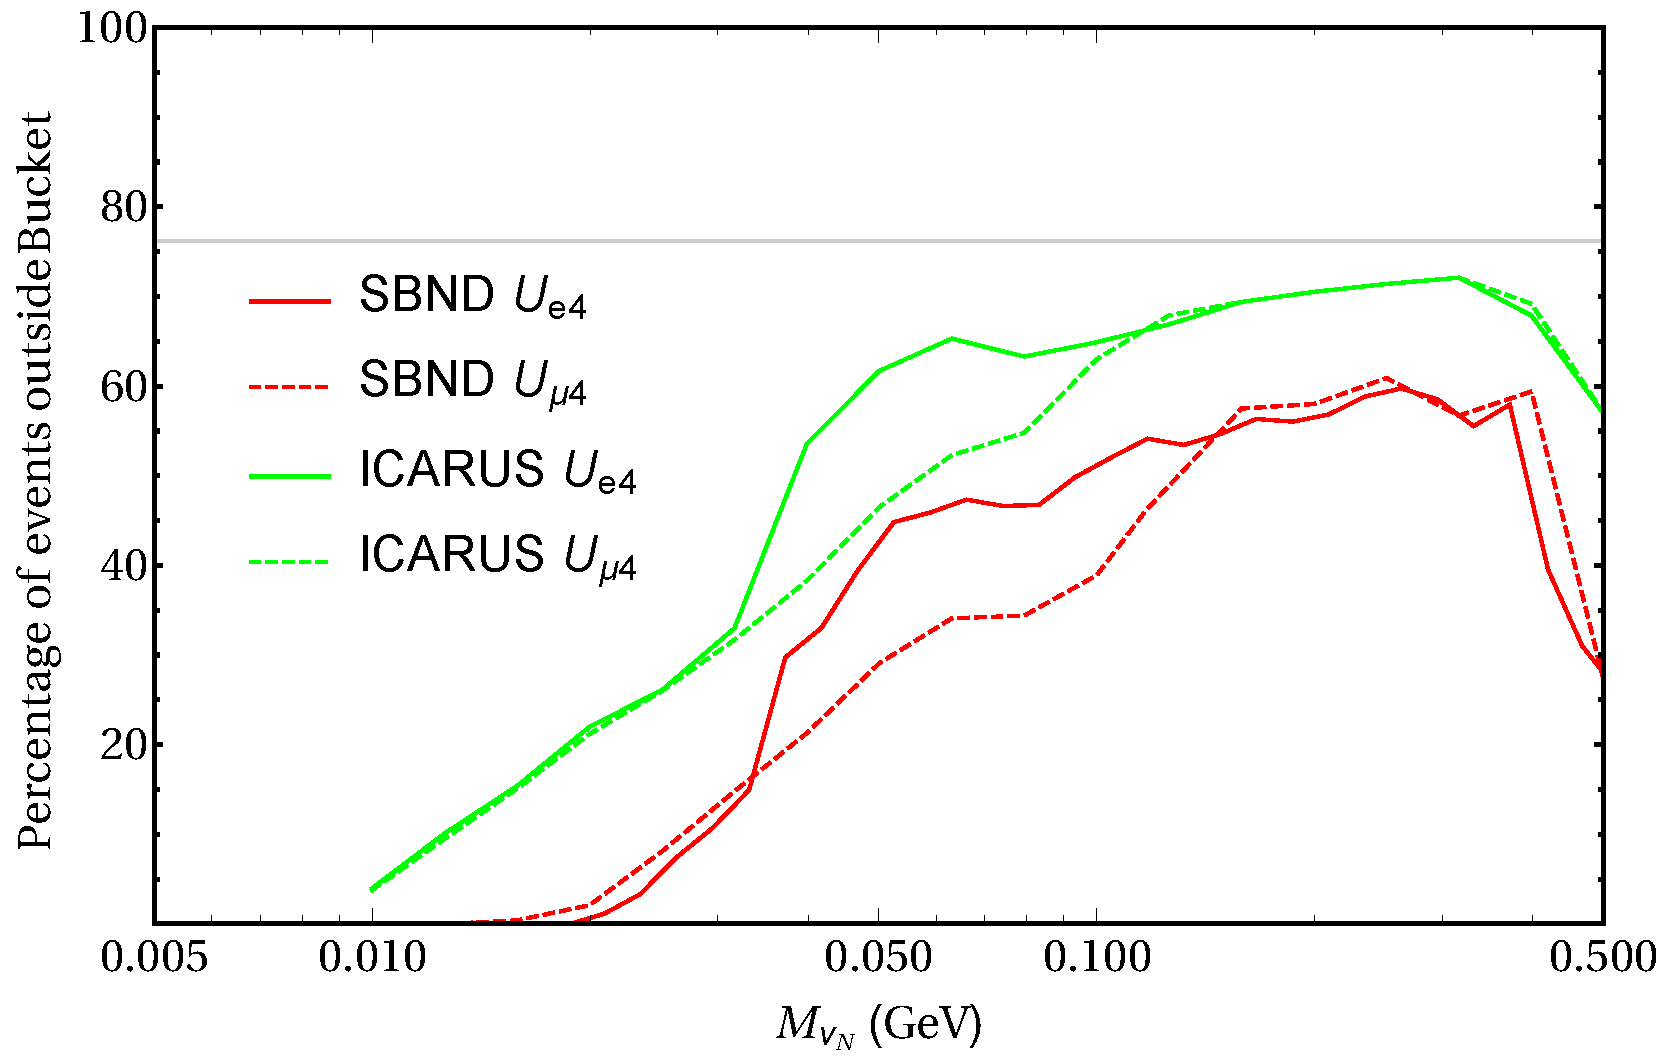
\includegraphics[width=0.7\textwidth]{figures/line_plots.pdf}
%
\caption{\label{fig:timing_line} The percentage of sterile decay events that fall into the inter-bucket region as a function of sterile mass for SBND and ICARUS, assuming a flux derived from $U_{e4}$ ($U_{\mu 4}$) mixing in solid (dashed) lines. Both SBND and ICARUS see a sizable fraction of total events outside the beam bucket windows when the sterile mass exceeds $\approx100$ MeV. The solid horizontal line corresponds to the percentage ($\approx 81$\%) if the events were uniformly distributed in time. (Running with more stats as we speak, but I do think its a good plot to have in some form or another)  
}
%
\end{figure}


The implication of the timing effects is that our discussion of backgrounds is twofold: for low mass steriles, or any mass at $\mu$BooNE due to timing resolution, we must consider all beam-related backgrounds as potential backgrounds. For larger masses at SBND and ICARUS, we may instead eliminate all signal events that lie in the bucket window and their associated beam-driven backgrounds and consider how to isolate the remaining signal events from the non-beam related background, predominately from cosmogenic events.

\section{Simulation details}
A crucial aspect of estimating the sensitivity of the SBN to sterile decays is accurate modeling of the incoming sterile fluxes. We have computed the fluxes and simulated event numbers for each beam and detector via a custom Monte Carlo program. The program allows efficiency's to be taken into account due to experimental details of the detector such as energy and timing resolution in a fully correlated way between observables. To leading order in the mass of the sterile neutrino over the pion, the fluxes
for the $\nu_N$ will be a rescaling of the fluxes for the active
neutrinos.  We take these neutrino fluxes as our input and scale them by the appropriate mixing $U_{\alpha 4}$, with an additional kinematic factor to take into account the helicity un-suppression of channels such as $\pi^+ \rightarrow e^+\nu_N$ for massive $\nu_N \gg m_e$. The flux of steriles produced from the decay of a meson M is therefore given by
\[
	\phi_{\nu_N}(E_{\nu_N}) \approx \phi_{\nu_\alpha} (E_{\nu_\alpha})\vert U_{\alpha 4}\vert^2 \frac{\rho\left( \delta_M^a , \delta_M^i \right)}{\delta_M^a \left(1- \delta_M^a\right)^2}.
\]
Where $\rho(a,b)=\mathcal{F}_M(a,b) \lambda^{\frac{1}{2}}(1,a,b)$ is a kinematic factor consisting of a term proportional to the two body phase space factor, $\lambda(x,y,z)=x^2+y^2+z^2-2(x y+yz+x z)$ and a term proportional to the matrix element, $\mathcal{F}_M(a,b)= a+b -\left(a-b\right)^2$, with $\delta_M^{a(i)}=m_{l_a(\nu_i)}^2/M^2$ \cite{PhysRevD.24.1232}. This kinematic effect for the pion and kaon can be substantial, in the case of $\pi \rightarrow e \nu$ this factor can be up to $10^5$, which more than compensates for the significantly smaller flux of $\nu_e$  inherent in the BNB. We only consider steriles below the kinematic threshold of the kaon (388 MeV for production via $|U_{\mu4}|$ mixing and 493 MeV for $|U_{e4}|$ driven production) as although there is a small component of heavier mesons such as the D meson which could produce heavier sterile states, they are produced in very small numbers due to the relatively low energy protons of the BNB beam. As the mass of the sterile increases, we begin to see components of the flux having energies less that the sterile mass, artificially loosing these events from the beam. In order to keep the normalisation of total neutrino events constant, before $U_{\alpha 4}$ and kinematic scaling, these events are shifted to be above the sterile mass threshold. \\

The neutrino fluxes at all three SBN detectors are calculated from published MiniBooNE fluxes \cite{AguilarArevalo:2008yp}, after scaling by appropriate $1/r^2$ baseline dependence, e.g $(470/540)^2 \approx 1.3$ at $\mu$BooNE. This is similarly scaled by $1/r^2$ for ICARUS at 600m, however, an additional energy dependant flux modifier is applied for SBND at 110m to account for the softer energy spectrum due to the proximity of the detector to the production target \cite{Antonello:2015lea}. We consider sources of neutrinos that are relavent including wrong sign neutrinos, smaller sub-dominant $K^+\rightarrow \pi^+\rightarrow \nu_\alpha$ as well as other contributions, predominately from meson decay chains initiated by meson-nucleus interactions, although all contributions other than neutrinos from two body meson decays are scaled by $|U_{\alpha 4}|^2$ only, not including the kinematic enhancement mentioned above. The neutrino spectrum at $\mu$BooNE is shown below in figure (\ref{fig:nuflux}). As the probability for any given sterile to decay scales as $1/E_N$, the fluxes at low energy are of particular importance. 

\begin{figure}[t]
\center
\begin{subfigure}[t]{0.5\textwidth}
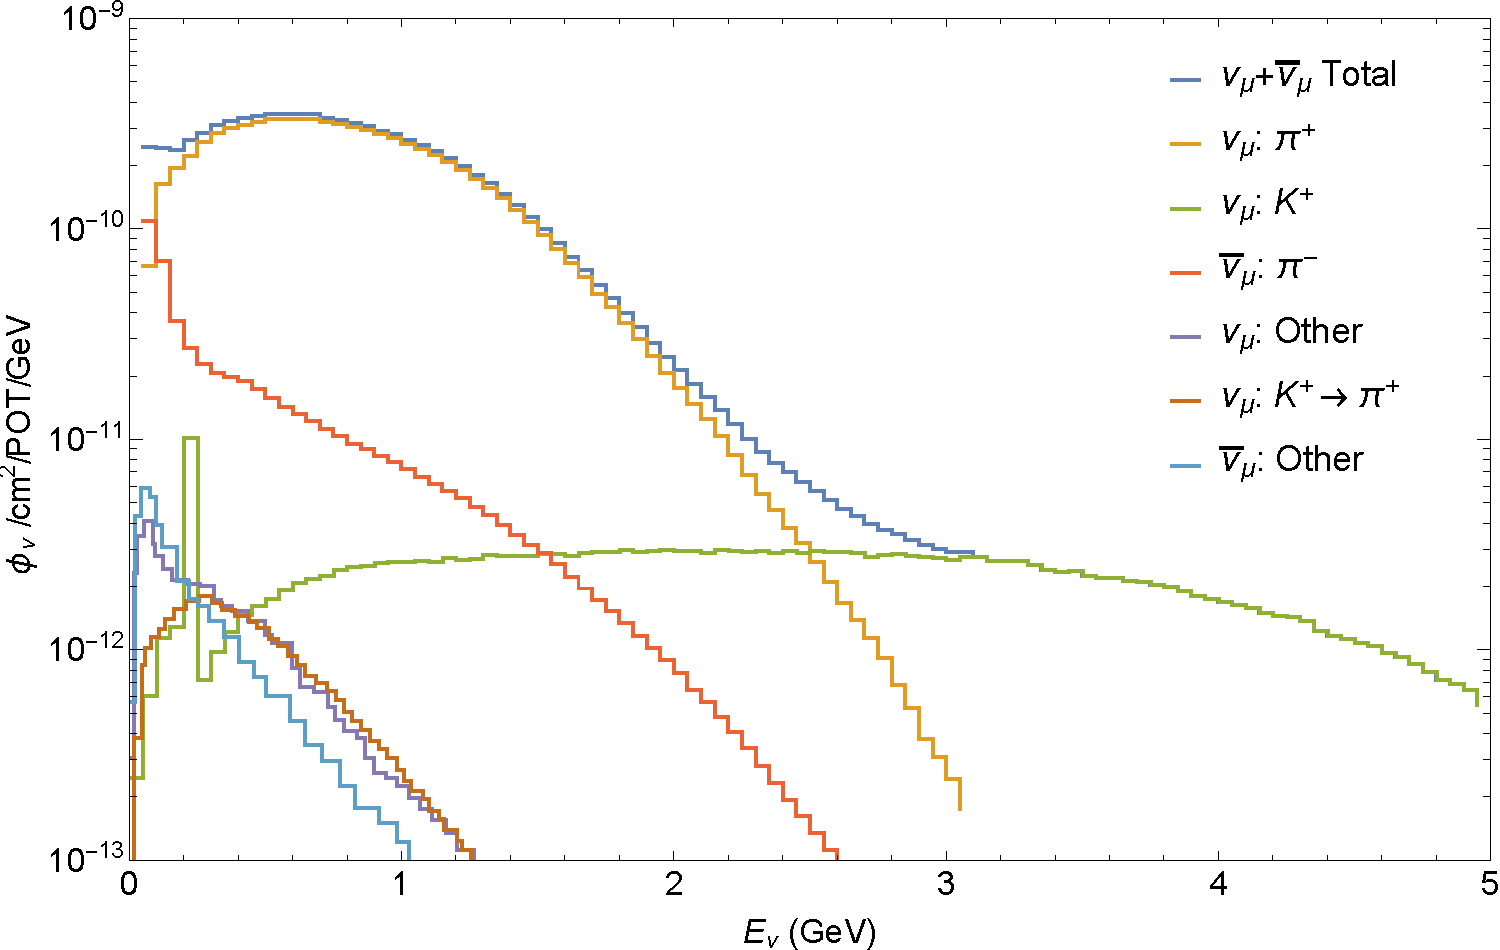
\includegraphics[width=\textwidth]{figures/microBooNE_flux.pdf} 
\end{subfigure}%
~
\begin{subfigure}[t]{0.475\textwidth}
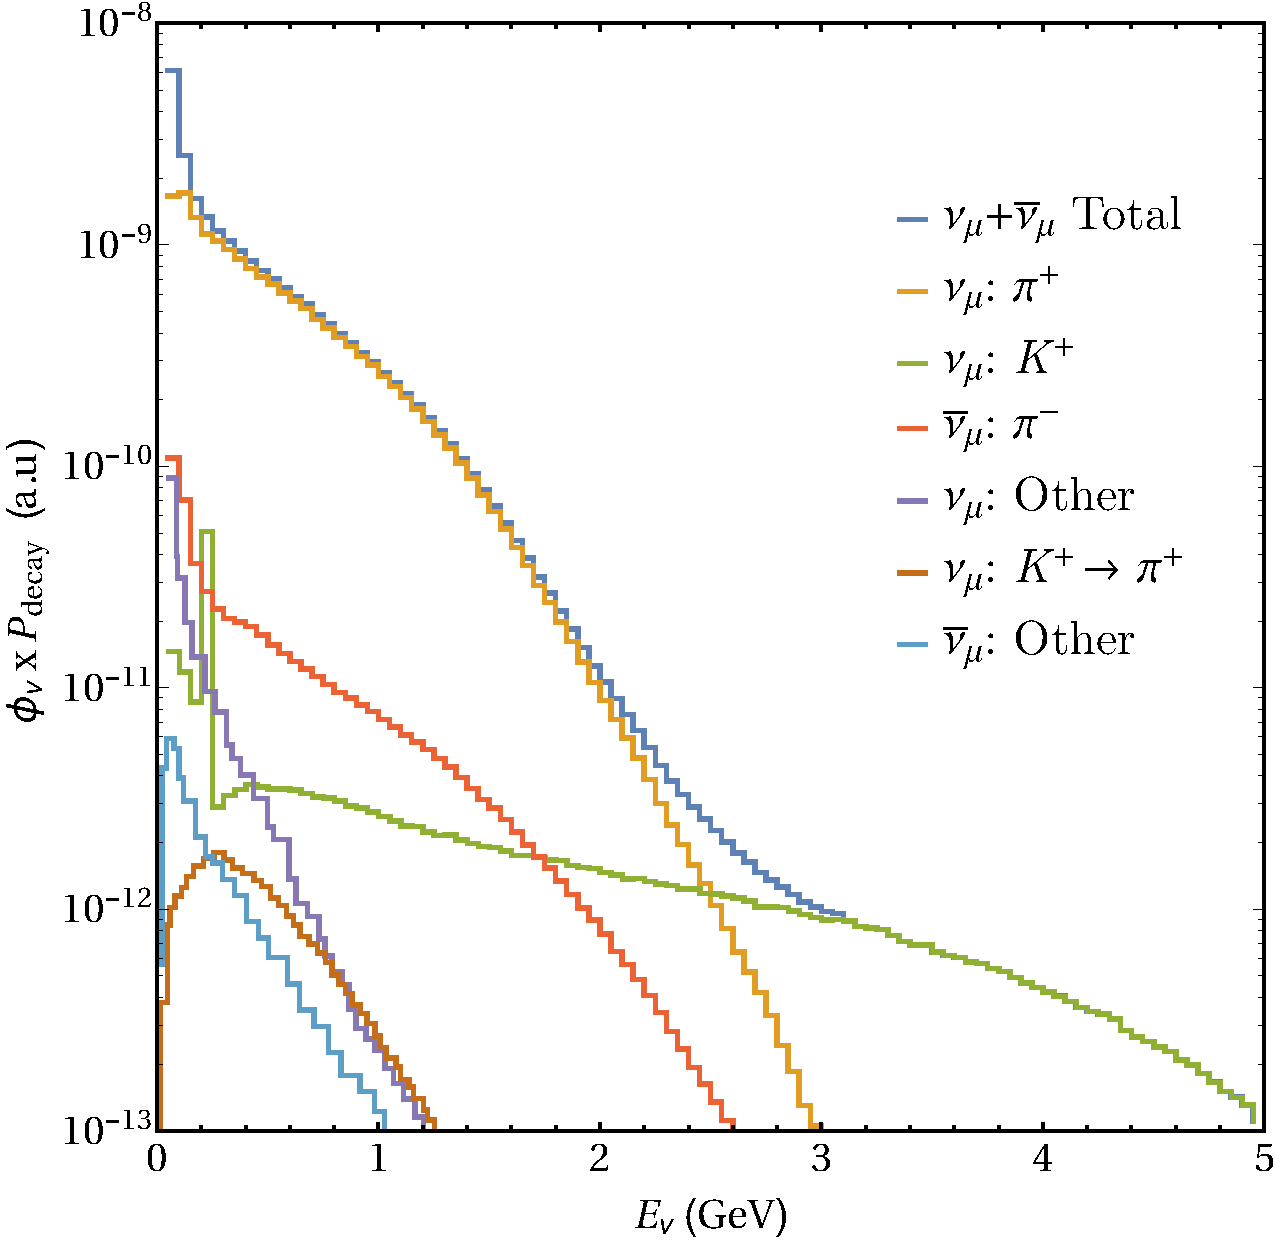
\includegraphics[width=\textwidth]{figures/microBooNE_flux_weighted.pdf}
\end{subfigure}
\caption{\label{fig:flux_plots} Left: The composition of fluxes of $\nu_\mu$ and $\overline{\nu}_\mu$ at $\mu$BooNE with horn in positive polarity (neutrino mode). ``Other'' refers to contributions primarily from meson decay chains initiated by meson-nucleus interactions. Right: Fluxes weighted by the probability to decay inside \muboone, for a sample 25 MeV sterile with equal $|U_{e4}|^2 = |U_{\mu 4}|^2$, and the horn in neutrino-mode. Requiring that the sterile decays has the effect of vastly increasing the importance of lower energy bins, where traditionally cross-section induced background effects are small.}

\end{figure}

\begin{figure}[t]
\center

\end{figure}

Given the spectral flux of sterile neutrinos in the BNB as calculated above, $\mathrm{d}\phi/\mathrm{d}E$, we compute the total number of accepted events in channel ``$\text{c}$'' via the following summation,
%
\[ N_\text{c} = \sum_{i} \left .
\frac{\mathrm{d}\phi}{\mathrm{d}E}\right|_{E_i} P_\text{D}\left(E_i\right)
W_\text{c}\left(E_i\right),  \]
%
where $P_\text{D}(E)$ is the probability for a sterile of that energy to reach
and then decay inside the detector labelled $\text{D}$. The simplest
approximation is to ignore all geometric effects, so that every particle
travels exactly along the direction of the beam line, which gives the following
probability 
%
\[ P_\text{D}\left(E\right) = e^{-\frac{\Gamma_\text{T}L}{\gamma\beta}}\left(
1-
e^{-\frac{\Gamma_\text{T}\lambda}{\gamma\beta}}\right)\frac{\Gamma_\text{c}}{\Gamma_\text{T}},
\label{eq:prob}
\]
%
where $\Gamma_\text{T}$ ($\Gamma_\text{c}$) denotes the rest-frame total decay
width (decay width into channel $\text{c}$), $m$ the mass of the sterile
neutrino, and $L$ ($\lambda$) the distance to (width of) the detector. The
combination $\gamma\beta$ is the usual special relativistic function of
velocities of the parent particle and provides the sole energy dependence of
the expression
%
\[   \frac{1}{\gamma\beta} \equiv \frac{m}{\sqrt{E^2-m^2}}. \]
%
As we are exploring a large parameter space, often this expression takes a
simplified form depending on the size of $\Gamma_\text{T}\lambda/\gamma\beta$:
%
\begin{align*} 
%
\Gamma_\text{T}\lambda \ll 1\qquad&\qquad P_\text{D} \approx
e^{-\frac{\Gamma_\text{T}L}{\gamma\beta}}\frac{\Gamma_\text{c}\lambda}{\gamma\beta}
+ \mathcal{O}\left(\Gamma_\text{T}^2\lambda^2\right),\\ 
%
\Gamma_\text{T}\lambda \gg 1\qquad&\qquad P_\text{D} \approx
e^{-\frac{\Gamma_\text{T}L}{\gamma\beta}}\frac{\Gamma_\text{c}}{\Gamma_\text{T}}
+ \mathcal{O}\left(\frac{1}{\Gamma_\text{T}\lambda}\right), 
%
\end{align*}
%
where the rate for slowly decaying particles can be seen to grow with detector
size until a width of $\lambda\sim\Gamma_\text{c}^{-1}$ where longer detectors
make no difference, as most steriles decay within a few decay lengths and
therefore we see a fixed fraction of the total events in our channel of interest. 

%
Finally, the function $W_\text{c}(E)$ is a weighting factor which accounts for
all effects which reduce the number of events in the sample: for example,
analysis cuts or detector performance effects.
%
To compute these factors, we run a Monte Carlo simulation of the decays for a
large number of sample events with a given energy. Each sterile event is
associated with a decay of type $\text{c}$. We then apply experimental analysis
cuts to the decays based on our assumptions about the detector's capabilities
and backgrounds, to produce a spectrum representing the final event sample. The
percentage of accepted events defines the weight factor for that energy. As such the full spectral shape of the signal is included in the rate analysis. As a consistency check of our methodology, we reproduce in Appendix (\ref{sec:ps191}) some
the published bounds of PS-191. 

%\newtext{PB}{We can compute all types of kinematic distributions to talk about
%cuts.} See \reffig{fig:ang_sep_E_total}.
%


%\begin{figure}[t]
%\center
%\includegraphics[width=1.0\textwidth,clip,trim=0 0 0 0]{figures/ang_sep_E_total_plot.pdf}
%
%\caption{\label{fig:ang_sep_E_total}The distribution of total energy deposited in an $e^+e^-$ pair from sterile neutrino decay in flight at \muboone\ against the apparent angular separation of the two particles.}
%
%\end{figure}
%
%
%\section{BNB Beam Timing}
%The above beam related backgrounds are relavent for lower mass steriles, $m_s \leq 50$ MeV and for highly boosted heavy steriles at SBND. Once the sterile becomes less boosted, however, the timing structure of the BNB becomes very relevant for which backgrounds dominate. The Booster neutrino beam consists of 81 Radio-Frequency(RF) buckets of approximately 2ns length, seperated by 19 ns, to form a 19.2$\mu$s spill with a frequency of 3Hz. All events inside this window, alongside all events in the surrounding bins according to an assumed 1ns resolution, are possibly beam-correlated. As can be seen in \ref{fig:timing} below, this is mainly true for light sterile neutrinos at all three SBN detectors, as well as a resonable approximation of heavy neutrino timings at SBND, however, $\mu$BooNE and ICARUS see significant deviation from this with clear peaks in the inter-RF-bucket spacing where one would not expect to see any beam-correlated backgrounds. \\
%
%Outside of the RF bucket timing window, where beam-driven backgrounds are relavant, one must have a very strong grasp of cosmogenics backgrounds. However, due to the high energy and very forwardness of the decay events, alongside the fact that one can observe the cosmogenic background in beam-off mode, gives us {\bf {\emph{faith}}} that one can get veyr close to backgroundless (Ya need to show this..). 
%
%The use of timing signals is significantly enhanced by the fact SBN has three detectors at varying baselines. If one observes an excess of events in SBND that appears consistant with a heavy sterile decaying in flight, this must correlate with a scaled number of events with an appropiate out-of bucket phase in both $\mu$BooNE and ICARUS. If this is not observed, one can rule out the decay in flight scenario.
%
%
%\begin{figure}[t]
%\center
%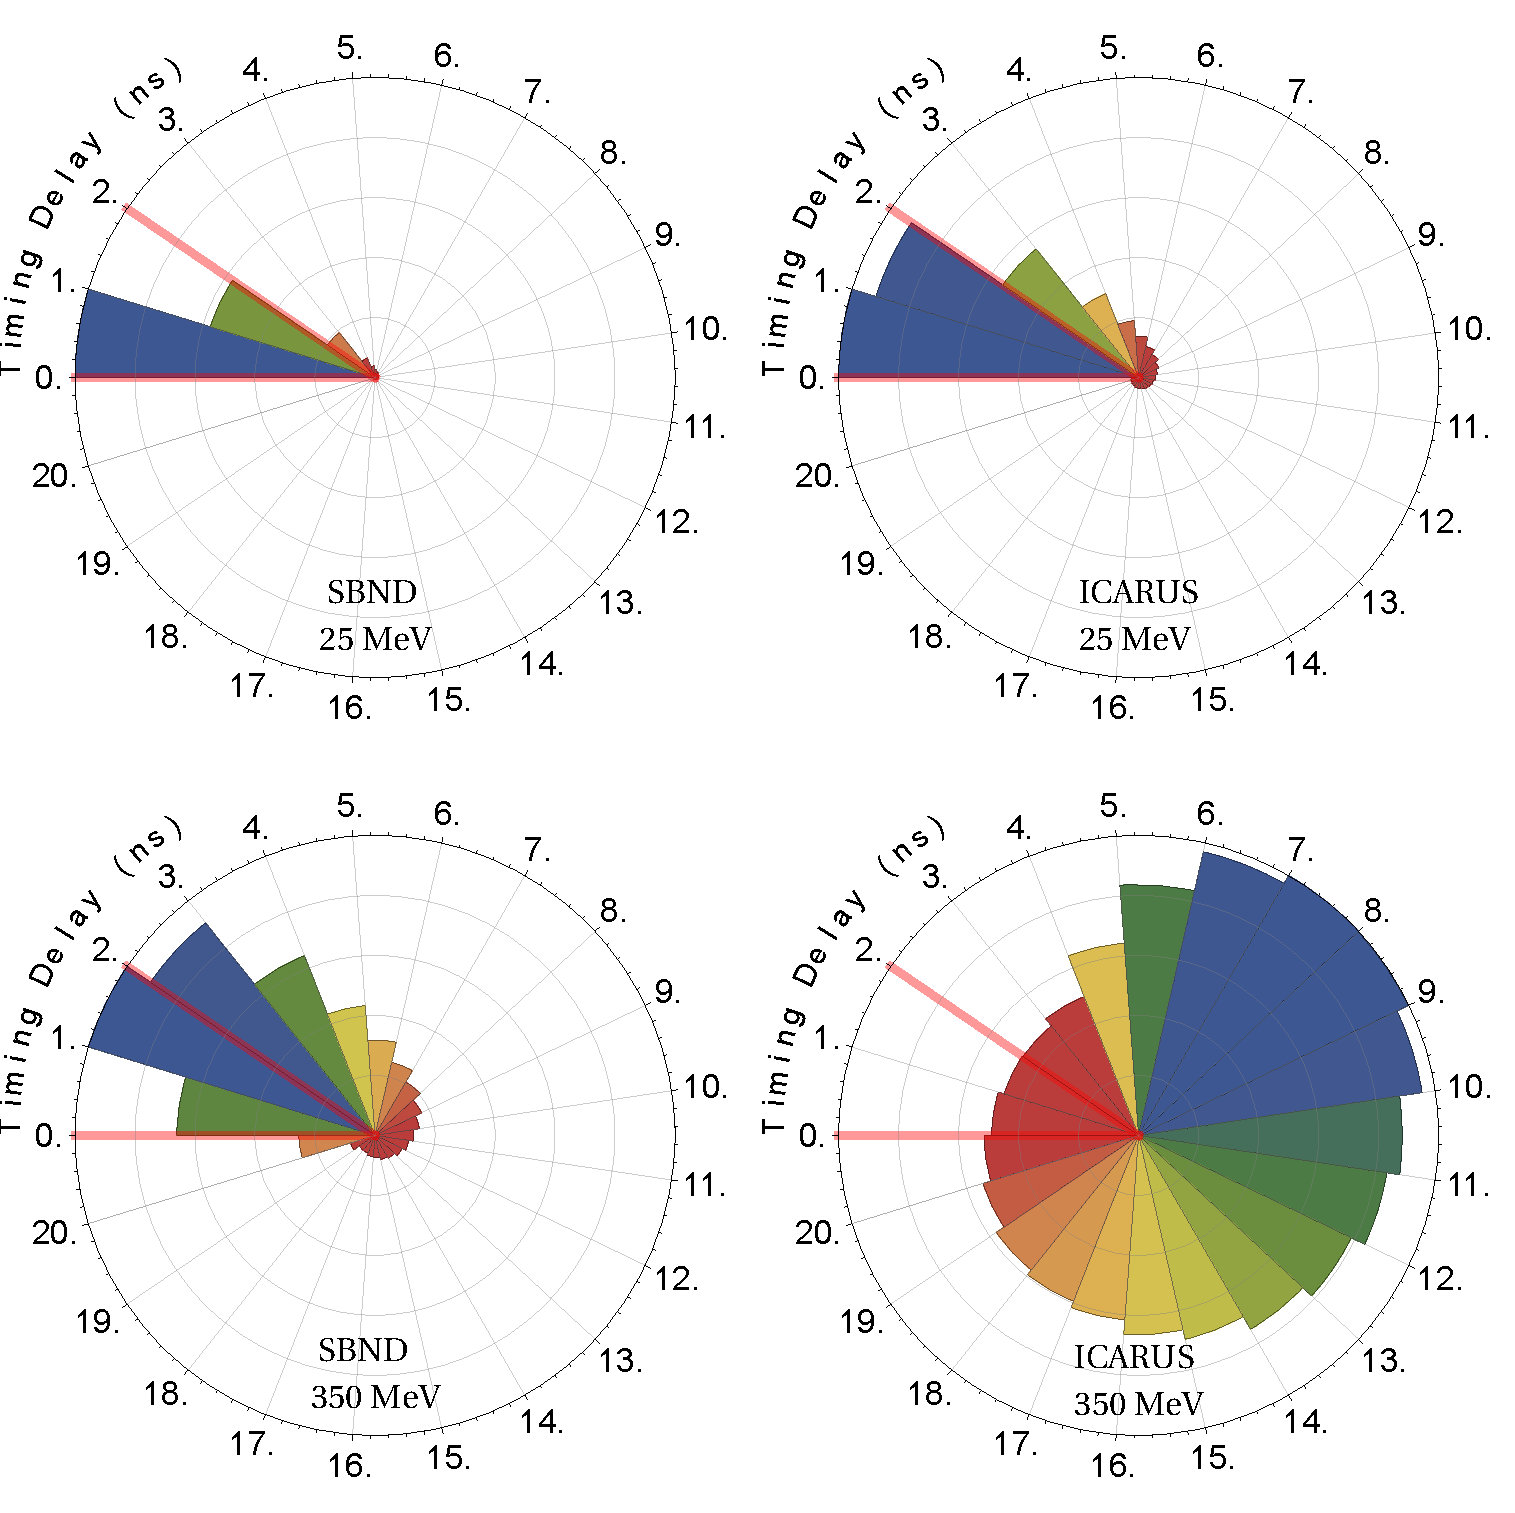
\includegraphics[width=\textwidth]{figures/timing.pdf}
%\caption{\label{fig:timing} Shown above is the timing delay of sterile neutrino decays in nano-seconds for both a 25 MeV (top) and 350 MeV (bottom) sterile neutrino at the SBND, $\mu$BooNE and ICARUS detectors (110,470 and 600m respectively). The 2 ns beam bucket window is shown highlighted in red from 0 to 2 ns, followed by an additional 19 ns gap. The timings are calculated as a difference relative to the time of flight of a active neutrino, assuming the decay occured in a uniform sample accross the 50m BNB decay pipe. A timing resolution of 1ns for all three SBN detectors is assumed to smear the observed events.}
%\end{figure}
%

\section{Sensitivities\label{sec:sensitivity}}
%
The results of our analysis are shown in \reffig{fig:band_sbn} below for the
combined SBN facility, and in \reffig{fig:band_sbn} for $\mu$BooNE for 6.6e20
POT, corresponding to 3 years running data . The lower colored lines show the
results of a backgroundless search, corresponding to the theoretical best
achievable sensitivity at the facility, assuming perfect signal efficiency. The
results of a simple cut based background analysis is also included as the upper
colored line. This background analysis is not optimsed, however, and serves
primarily to show the potential impact of backgrounds, see Appendix
(\ref{sec:bg}) for details of the backgrounds included in this analysis. We
estimate the true achievable sensitivity in each channel would lie somewhere
between these two curves (the solid shaded region). The analysis only considers
the total number of events in each channel, with the 90\% C.L defined as $2.44$
events, following the procedure of \refref{Feldman:1997qc} designed for
backgroundless searches for rare events. For the backgroundless search the
representative quantity $S/\sqrt{B}$ is contoured for a direct comparason.  \\

As can be seen SBN potentially sees significantly more events that PS-191, and
thus could improve the bounds for large sections of parameter space in all
channels and on all mixing elements. \muboone\ is slightly better than the
corresponding PS191 bounds for low mass steriles (due to the lower energy
neutrino spectrum) and approximately equal at higher masses. The previously
unbounded $\nu_N \rightarrow \nu_\alpha \pi^0$ can potentially be bounded at a
level very similar to the previous PS-191 $e^+ e^-$ channel. 

\begin{figure}[t]
\center
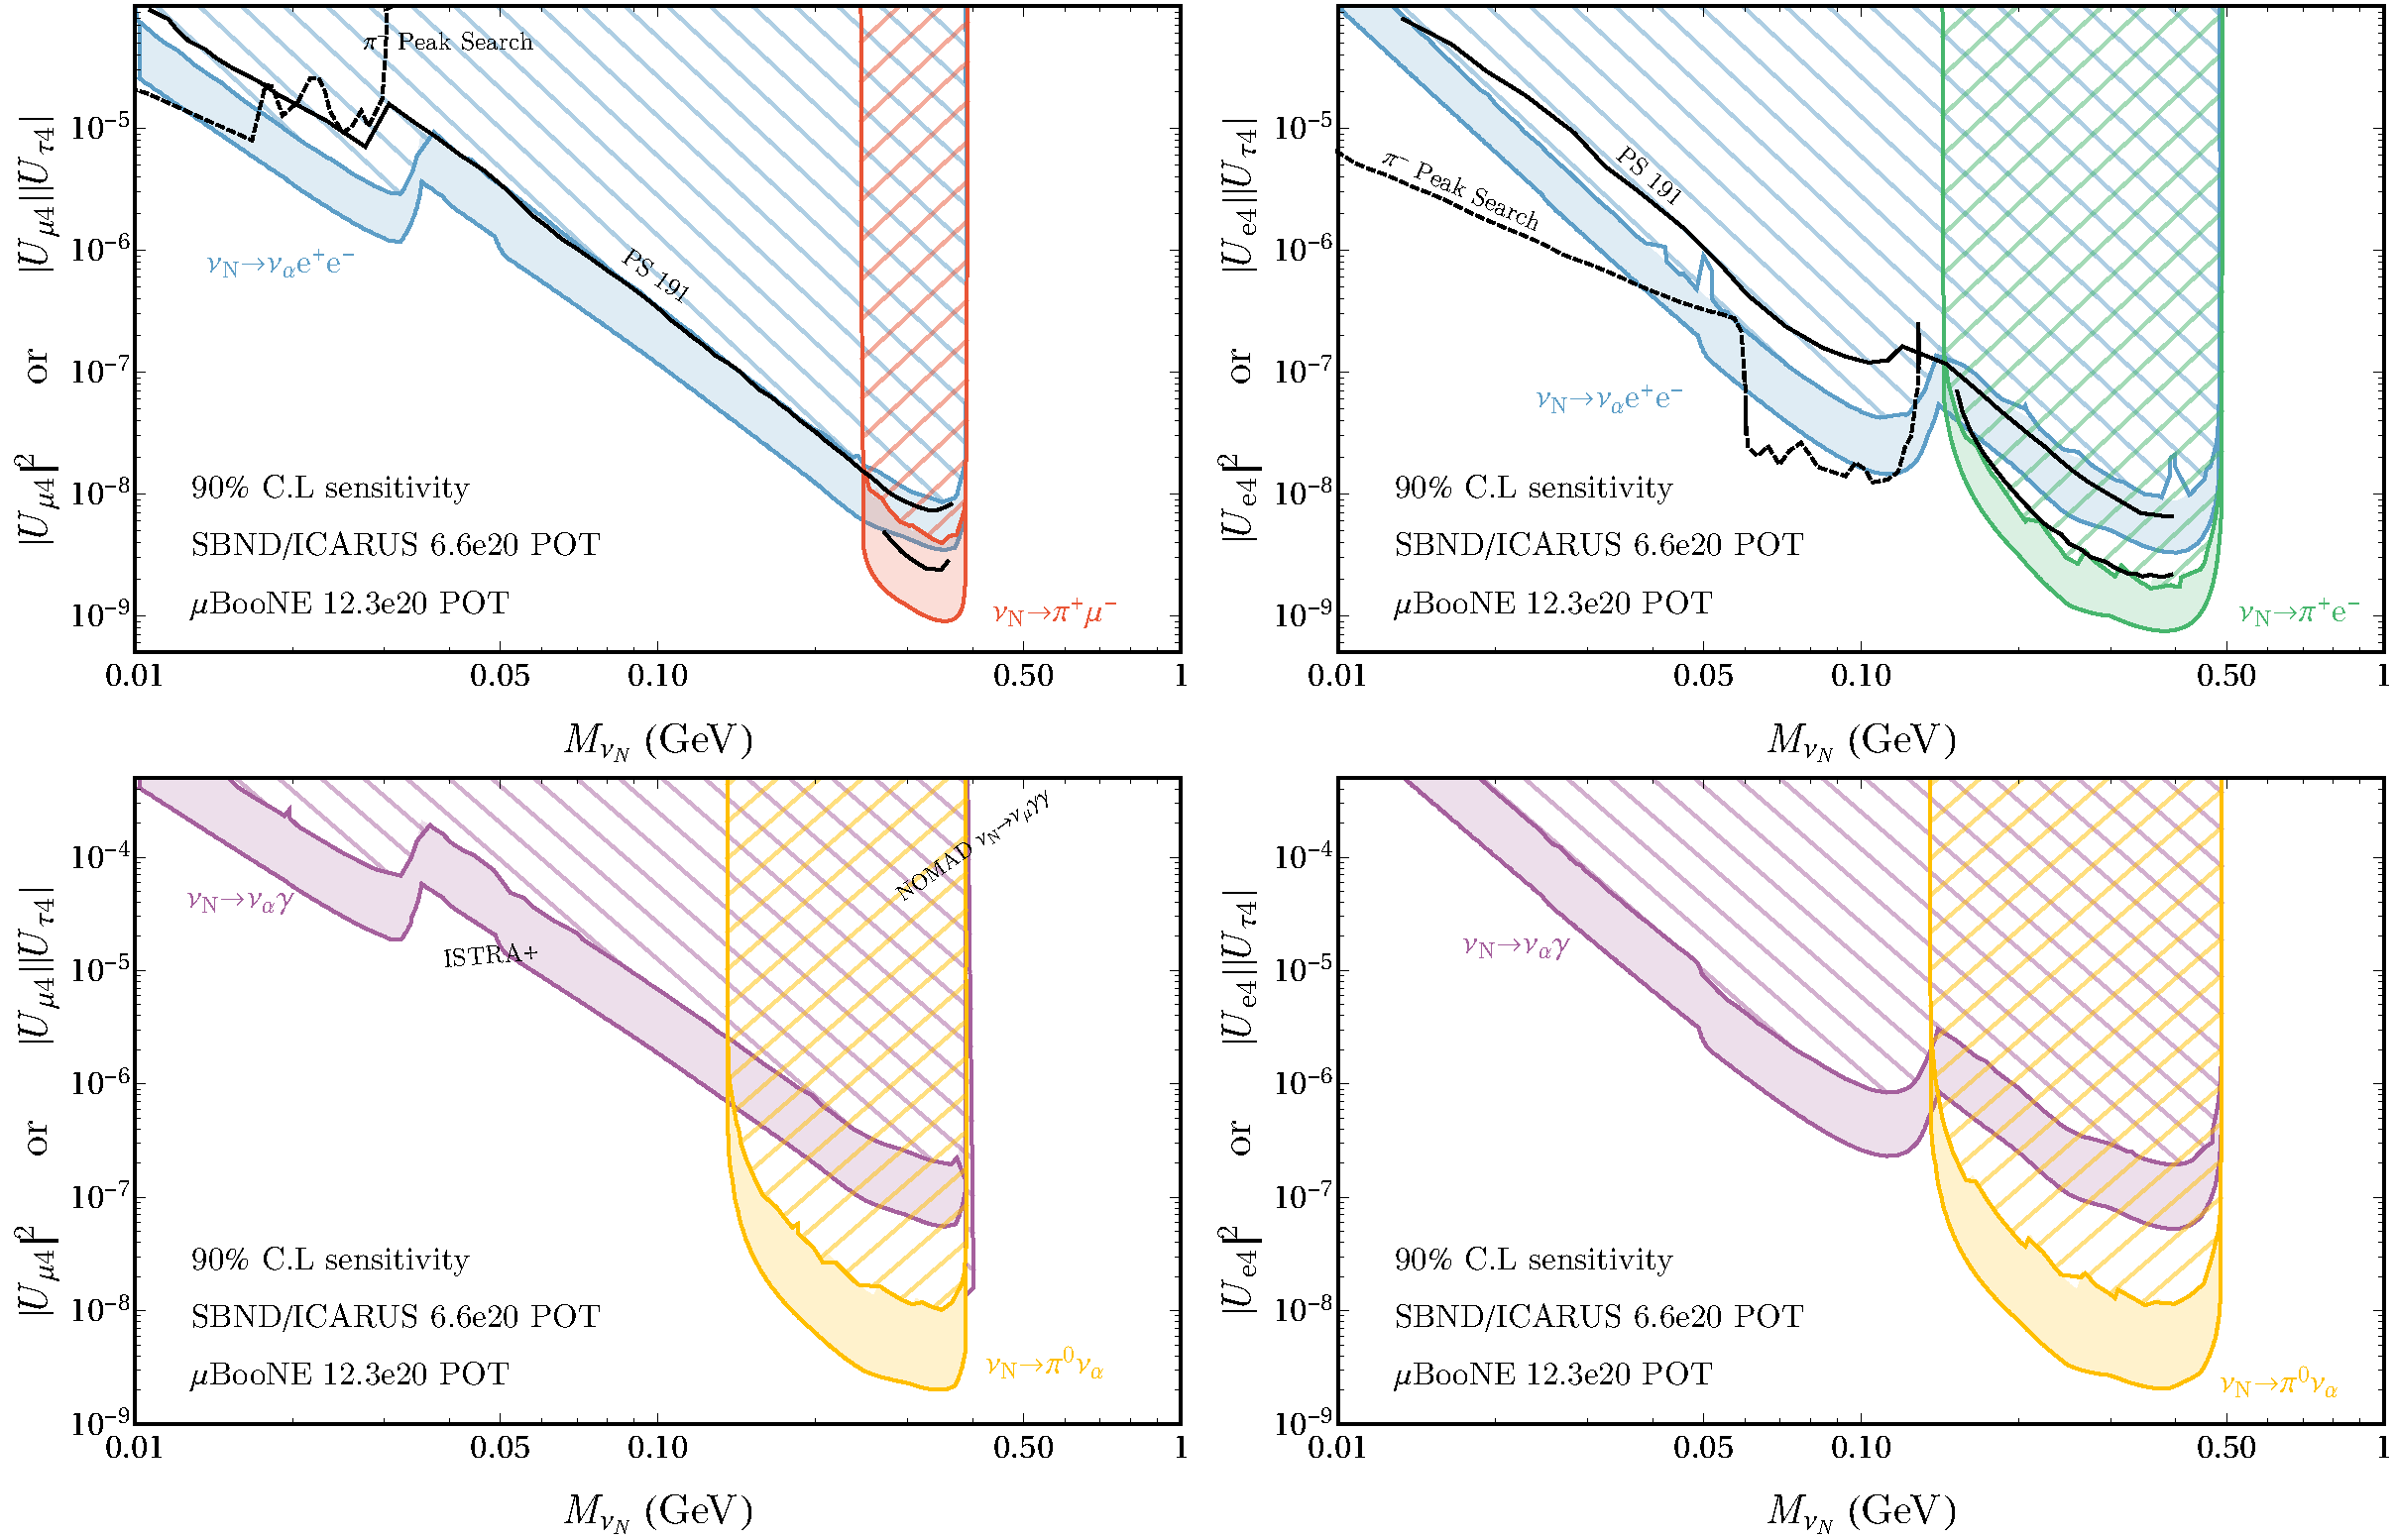
\includegraphics[width=1.0\textwidth]{figures/band_sbn.pdf}

\caption{\label{fig:band_sbn}The sensitivity contours for the combined SBN
facility. Shown also in black solid lines is the prior best bounds from PS-191,
scaled to show bounds on the minimal extension as discussed here. In all
panels, the mixing matrix elements not shown on the $y$-axis are zero. Above we
have the previously bounded channels, $e^+e^-$ and $l^- \pi^+$ for nonzero
$U_{\mu 4}$ and $U_{e4}$ respectively. Below we have the same for the unbounded
$\gamma$ and $\pi^0$ channels.}

\end{figure}

\begin{figure}[t]
\center
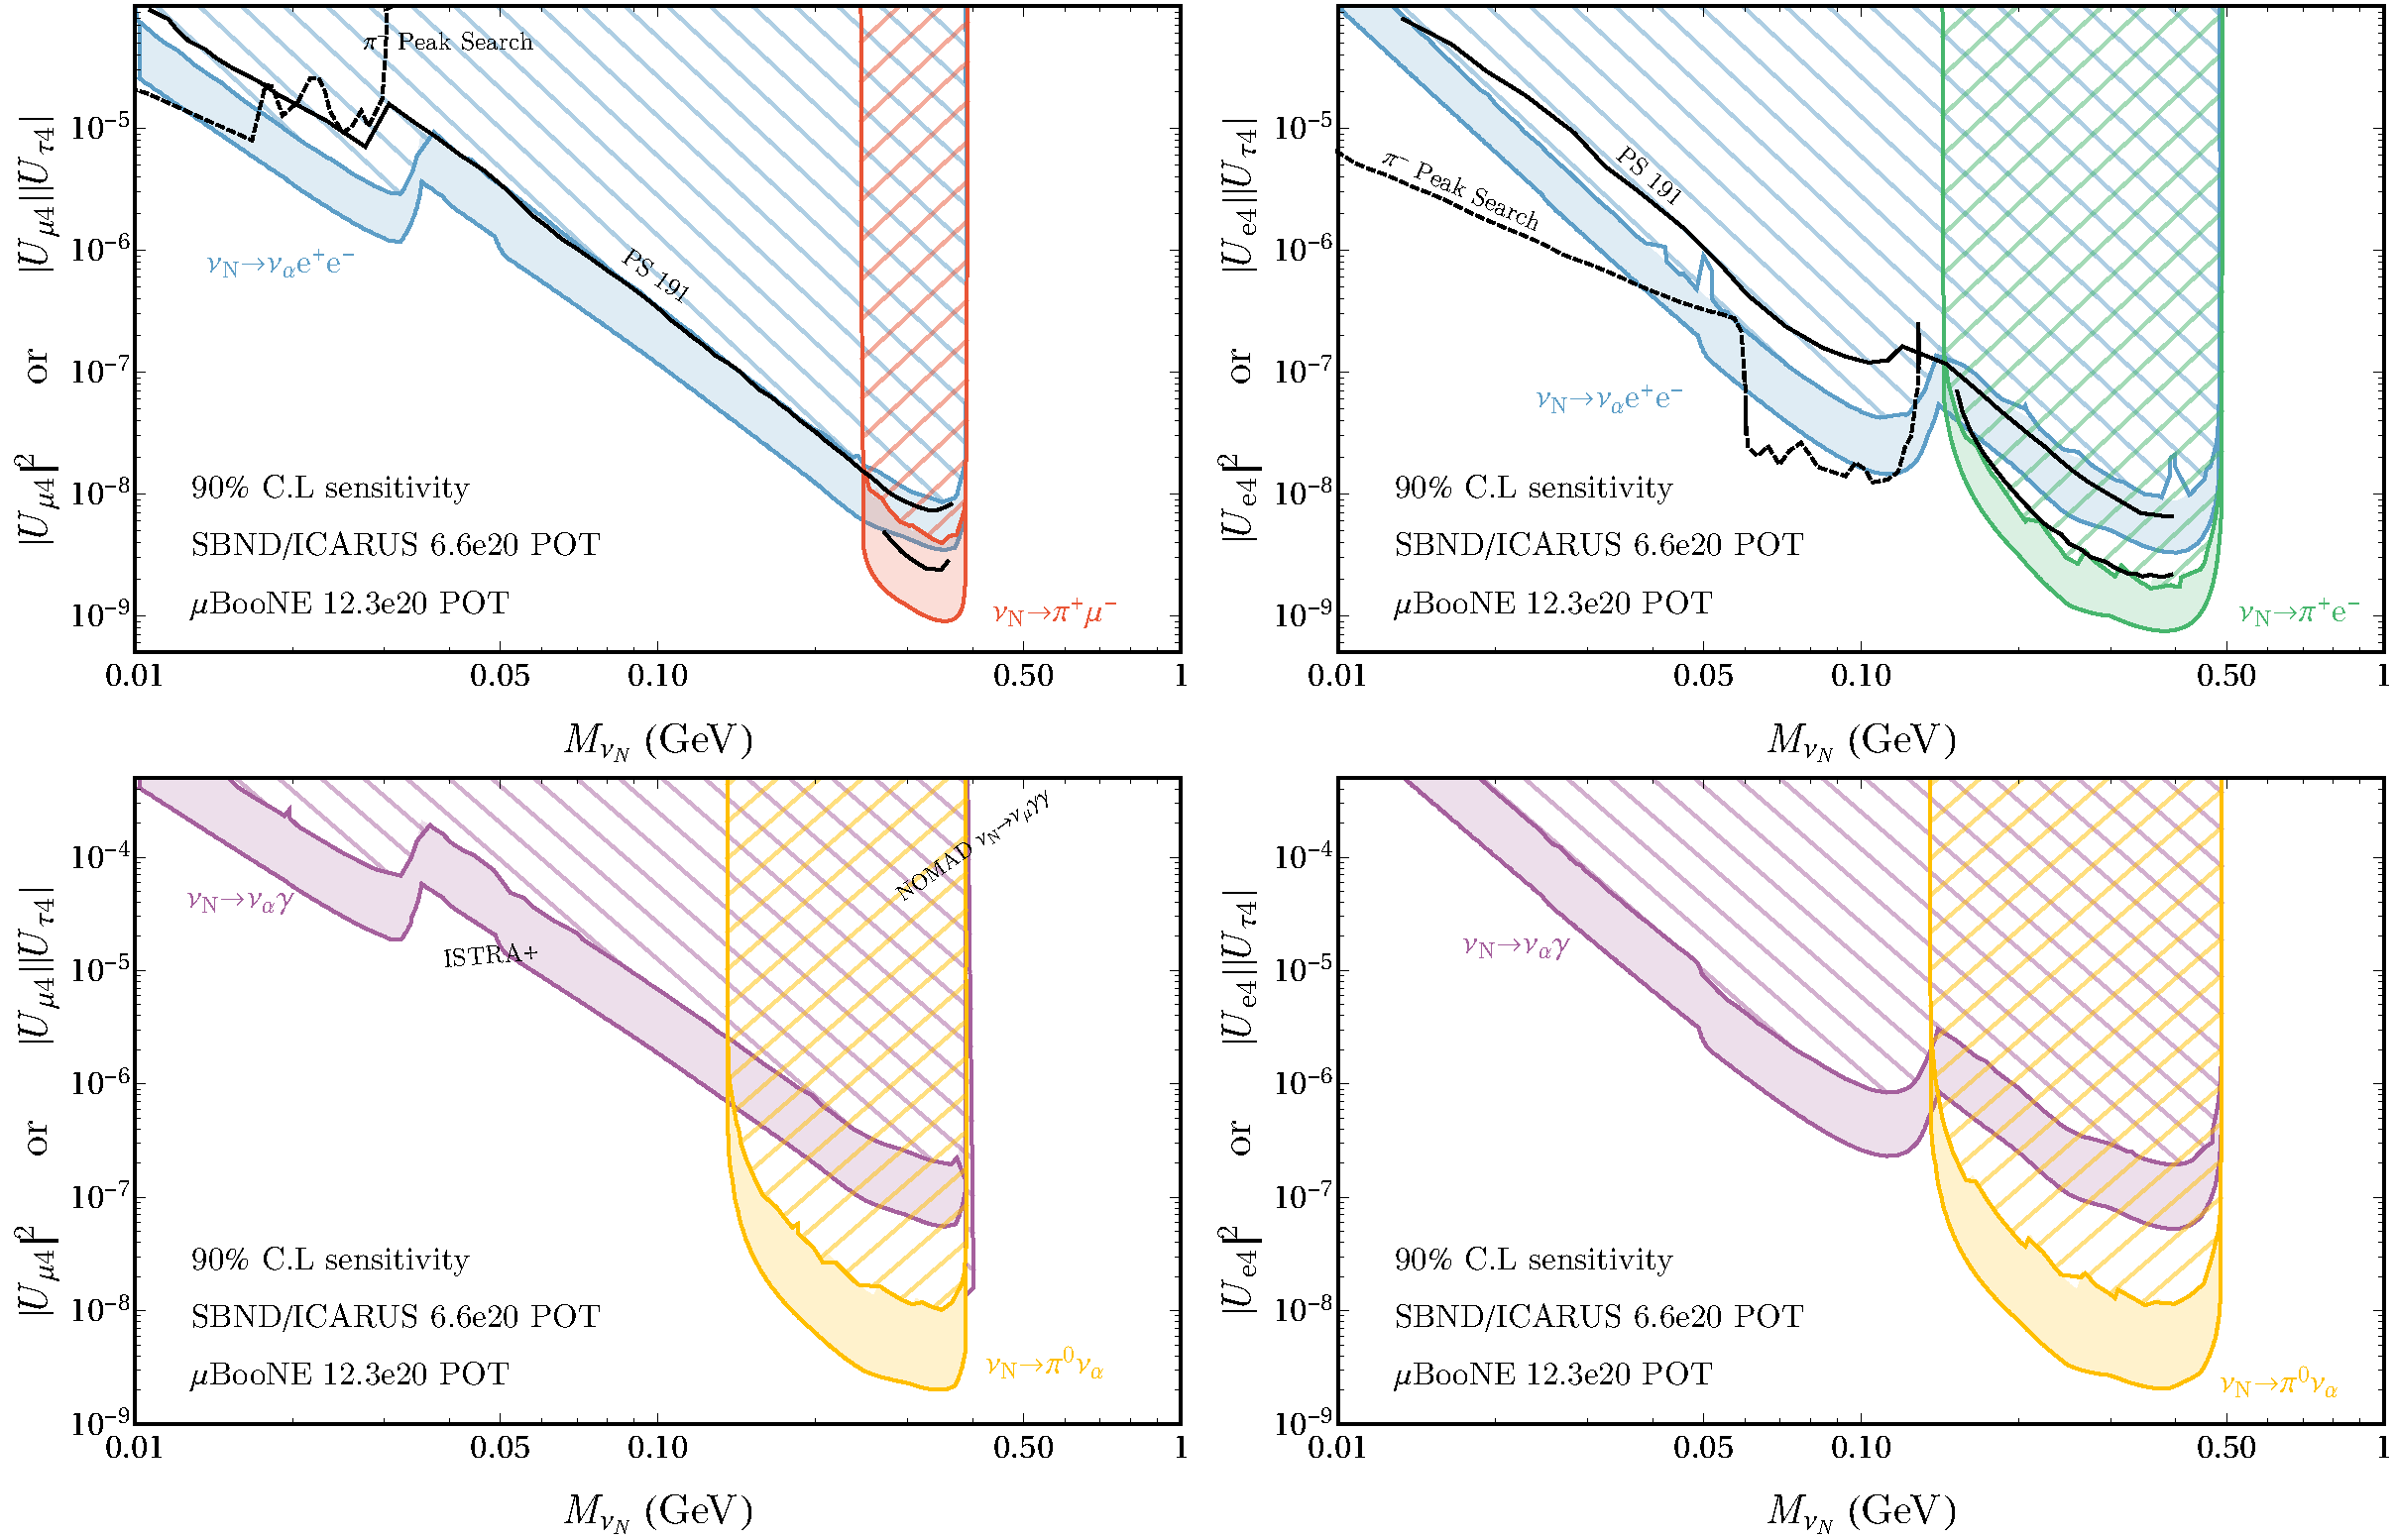
\includegraphics[width=1.0\textwidth]{figures/band_sbn.pdf}

\caption{\label{fig:band_muboone} PLACEHOLDER: The sensitivity contours for the
$\mu$BooNE alone with  3 year running in neutrino mode, $6.6\times 10^{20}$
POT. Shown also in black solid lines is the prior best bounds from PS-191,
scaled to show bounds on the minimal extension as discussed here. In all
panels, the mixing matrix elements not shown on the $y$-axis are zero. Above we
have the previously bounded channels, $e^+e^-$ and $l^- \pi^+$ for nonzero
$U_{\mu 4}$ and $U_{e4}$ respectively. Below we have the same for the unbounded
$\gamma$ and $\pi^0$ channels.}

\end{figure}


%In order to facilitate the search for new physics we provide results in terms
%of a total scaling $\Gamma$, of each decay channel of interest. We retain the
%functional dependance on sterile mass as in the minimal, bounding $\Gamma \vert
%U_{\alpha 4}\vert^2$. \\

%standard model weak processes with an active mixing scaling. Beyond this there
%are many extensions worth considering, if the sterile sector is charged under a
%new gauge symmetry, e.g $U(1)'$, then the total decay rate can be significantly
%modified. Additional new particle content that couples strongly with the sterile
%states can also drastically change the expected rate with respect to the minimal
%extension, as well as open up entirely new decay channels, such as the possible
%radioactive decay $\nu_N \rightarrow \nu_\alpha \gamma$, which can also be probed
%at the SBN and provides a window to searches for large sterile magnetic
%moments. In order to facilitate the search for new physics we provide results
%in terms of a total scaling $\Gamma$, of each decay channel of interest. We
%retain the functional dependence on sterile mass as in the minimal, bounding
%$\Gamma \vert U_{\alpha 4}\vert^2$. \\

%If there was an enhancement of $\alpha$ in a single channel, $\Gamma_c$, such
%that the total decay width becomes $\Gamma_\text{tot} =
%\Gamma_\text{oth}+\Gamma_c (1+\vert U_{\mu 4}\vert^2 \alpha)$, then previous
%experiments searching for heavy sterile decays would have had much more
%stringent bounds on $\vert U_{\mu 4} \vert^2$. We can estimate these enhanced
%bounds by comparing the probability to decay in a particular channel, with the
%probability associated with the published bounds, in particular we need to find
%the new value for the 90\% C.L bound, $\vert U_{\mu 4}\vert^2$, such that the
%probability to decay inside a detector of baseline L and length $\lambda$, with
%a total rate  $\Gamma_\text{tot} = \vert U_{\mu 4}\vert^2
%\left(\Gamma_\text{oth}^\prime+\Gamma_c^\prime (1+\alpha)\right)$, is equal to
%the probability to decay inside the same detector with total rate
%$\tilde{\Gamma}_\text{tot} = \vert U_{\mu 4}^*\vert^2(m_S)
%\left(\Gamma_\text{oth}^\prime+\Gamma_c^\prime\right)$, where $\vert U_{\mu
%4}^*\vert^2(m_S) $ indicates the published bound on that channel, for a sterile
%of mass $m_S$, and primed decay widths indicate the width with mixing removed
%to the front. Using the functional form of the probability in equation
%\ref{eq:prob}, and expanding to leading order in the assumed small parameter
%$\lambda/L$, there are two solutions to this corresponding to the two real
%branches of the Lambert-W function. The two solutions correspond physically to
%the cases where an increasing decay rate increases the number of observed
%events in a detector thus increasing the bound, $\mathcal{W}_0$, up until the
%decay rate becomes sufficiently large to ensure the majority of the events
%decay before reaching the detector, $\mathcal{W}_{-1}$. This places the 90\%
%C.L exclusion in a region \[	-\frac{\vert U_{\mu 4}^* \vert^2}{ \kappa
%\Gamma_\text{tot}^{*}} \mathcal{W}_{-1} \left[-\frac{\kappa
%\Gamma_\text{tot}^{*}}{1+\alpha} \exp\left(
%-\kappa(\Gamma_c^*+\Gamma_\text{oth}^*) \right)     \right]	\geq \vert
%U_{\mu 4} \vert^2 \geq \frac{\vert U_{\mu 4}^* \vert^2}{1+\alpha} \] where
%$\kappa = \frac{L}{\gamma \beta}$ and we have expanded $\mathcal{W}_0$ to
%leading order in $\vert U_{\mu 4}^*\vert^2$ for clarity to see it scales as
%expected with enhancement $(1+\alpha)$ , no such convenient expansion exists
%for  $\mathcal{W}_{-1}$.  

% 
%\begin{figure}[t]
%%
%\centering
%%
%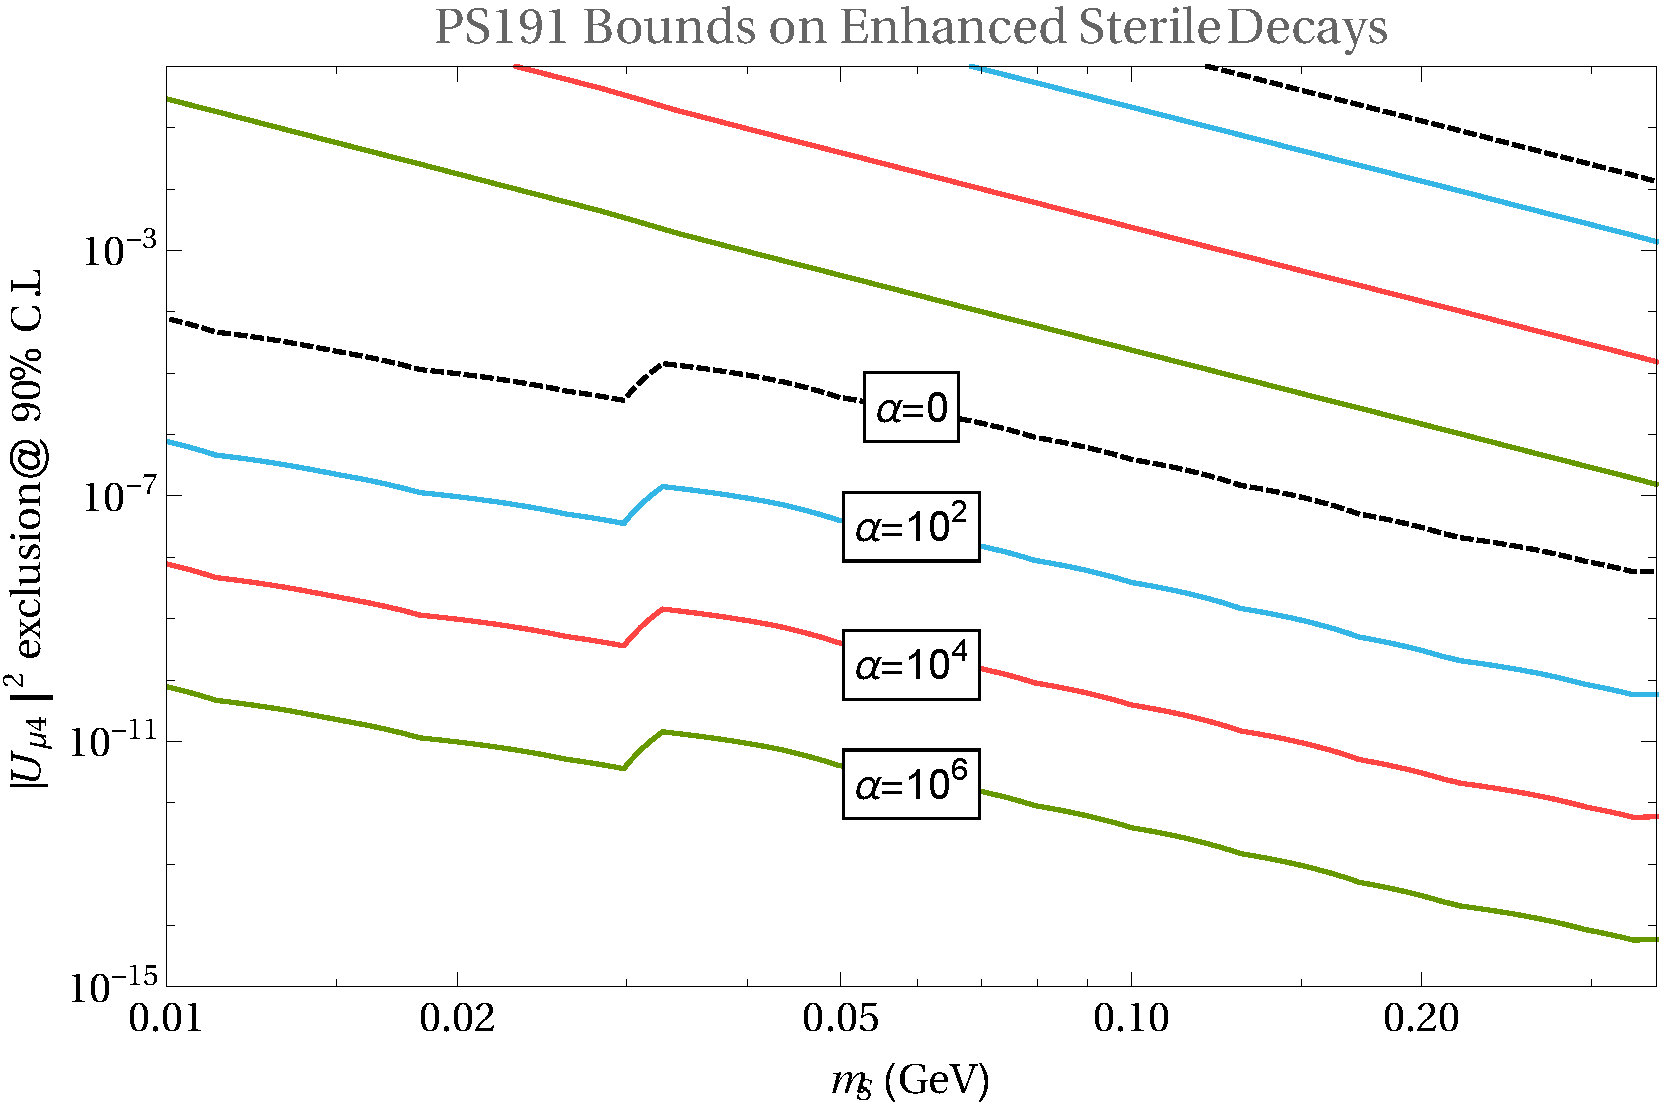
\includegraphics[width=0.49\textwidth]{figures/ps191_enhanced.pdf} 
%%
%\caption{\label{fig:ps191_enhance}The shifting of bounded region (excluded at
%90 \% C.L  between coloured line pairs) as the decay rate to a specific channel
%($\nu_N \rightarrow \nu_\mu e^+e^-$) is increased by an arbitrary scaling
%factor $\alpha$ at the PS-191 facility,$\alpha = 0$ corresponds to the minimal
%model bounds. A baseline of 128m, and mean energy of $\left< E_\nu \right>
%\approx 1 GeV$ was assumed.  , as well as the }
%%
%\end{figure}
%To investigate how the presence of backgrounds weaken these sensitivities, we
%have performed a rough estimate of the significance of the signal in various
%channels. In \reffig{fig:no_cuts_scaled_bkg}, we consider the quantity
%$S/\sqrt{\lambda B}$ and plot contours when the parameter is equal to $1$. At
%this point, the size of the new signal events from the heavy sterile decays are
%equal to the Poisson noise in the experiment under the approximation of no
%signal. The parameter $\lambda$ is used to scale the backgrounds, corresponding
%to a greater ability to suppresses these events.  We show two regions, the most
%conservative line corresponds to $\lambda=1$ with no additional background
%suppression beyond our estimates, whilst the more optimistic one corresponds to
%a further suppression by a factor of 1000. Our estimates are given by the
%largest numbers in \reftab{tab:rates} for each channel, that is assuming no
%analysis-based reduction in rates. As before, we do not take into account the
%signal efficiency in these plots (weight factors are set to $1$) this makes the
%unrealistic assumption that whatever has been done to reduce the backgrounds
%leaves the signal event rates unchanged. However, it provides an understanding of 
%the severity of the impact of the backgrounds for these searches.
%
%\newtext{PB}{Be careful: the contours aren't really the same thing as the
%shaded region, as they are computing different statistical quantities. But to
%make them into actual exclusion curves, we would have to minimize over the 2D
%space... which maybe we should do... but as we know it takes a bit of work.
%Also, the ee flux isn't quite right for a reason I forget at the moment.}
%
%
%\begin{figure}[t]
%\center
%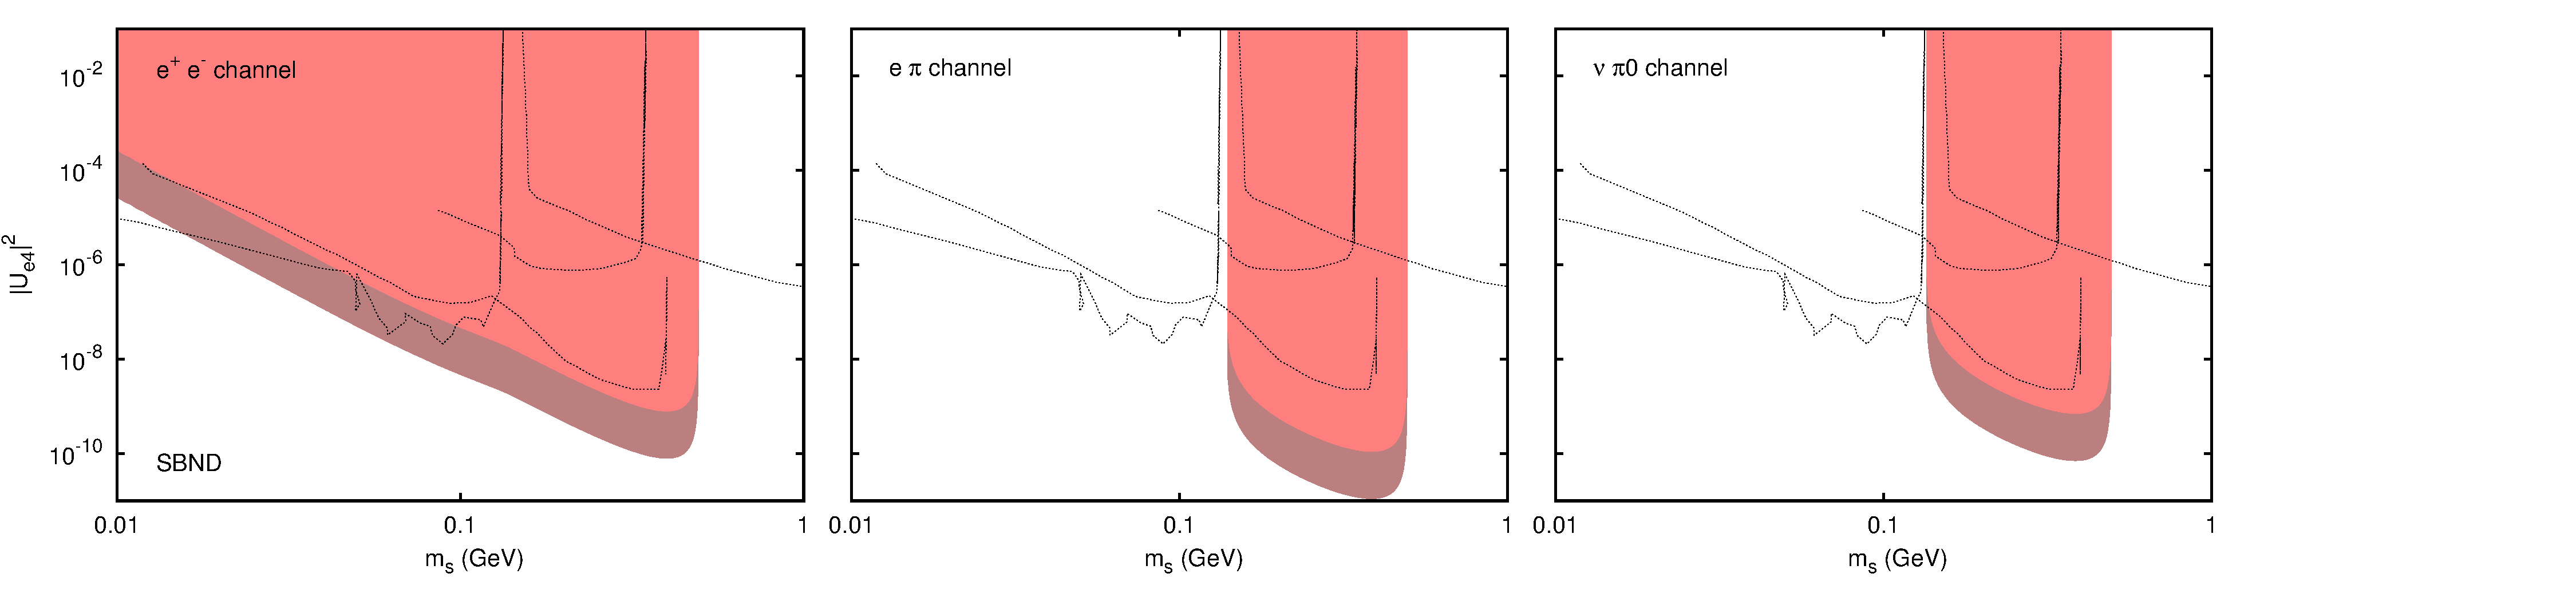
\includegraphics[width=1.0\textwidth,clip,trim=0 20 300 15]{figures/sbnd_all_panels_ue4.pdf}
%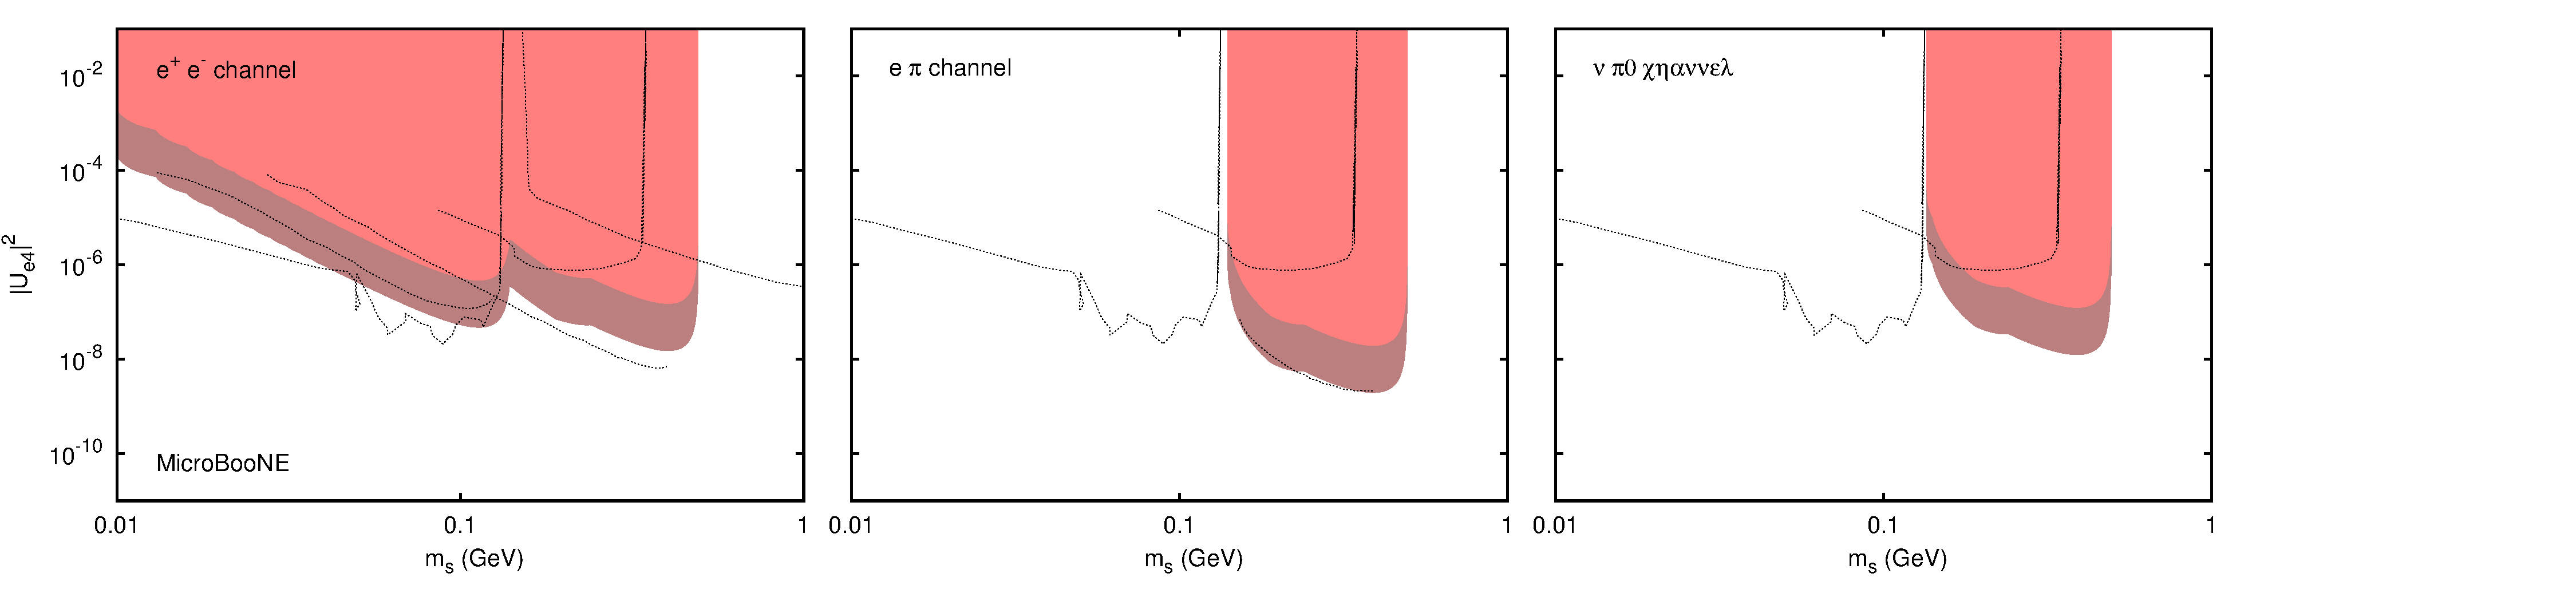
\includegraphics[width=1.0\textwidth,clip,trim=0 20 300 15]{figures/muboone_all_panels_ue4.pdf}
%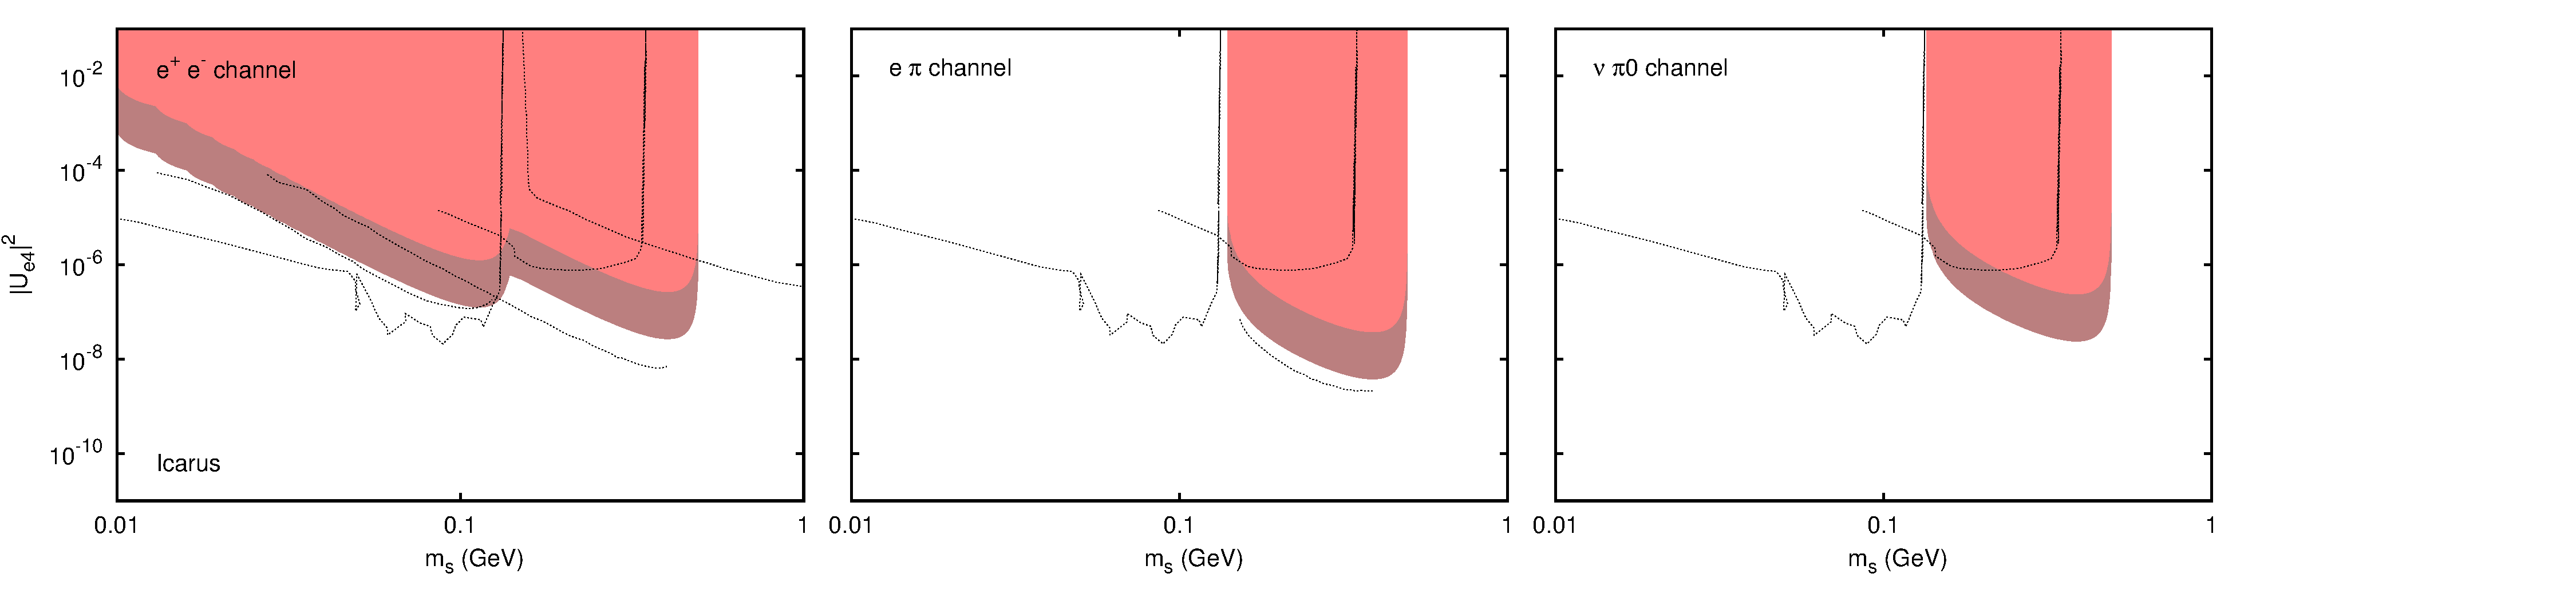
\includegraphics[width=1.0\textwidth,clip,trim=0 20 300 15]{figures/icarus_all_panels_ue4.pdf}
%
%\caption{\label{fig:no_cuts_scaled_bkg_ue4_only}The sensitivity contours based on the total
%	number of events, assuming only mixing with the electron neutrino ( $\vert U_{\mu 4}\vert^2=\vert U_{\tau 4}\vert^2=0$), without cuts but with varying degrees of background
%suppression. We overlay the 95\% exclusion regions for $U^2$ and $m_s$ from
%previous experimental work.}
%
%\end{figure}
%
%\begin{figure}[t]
%\center
%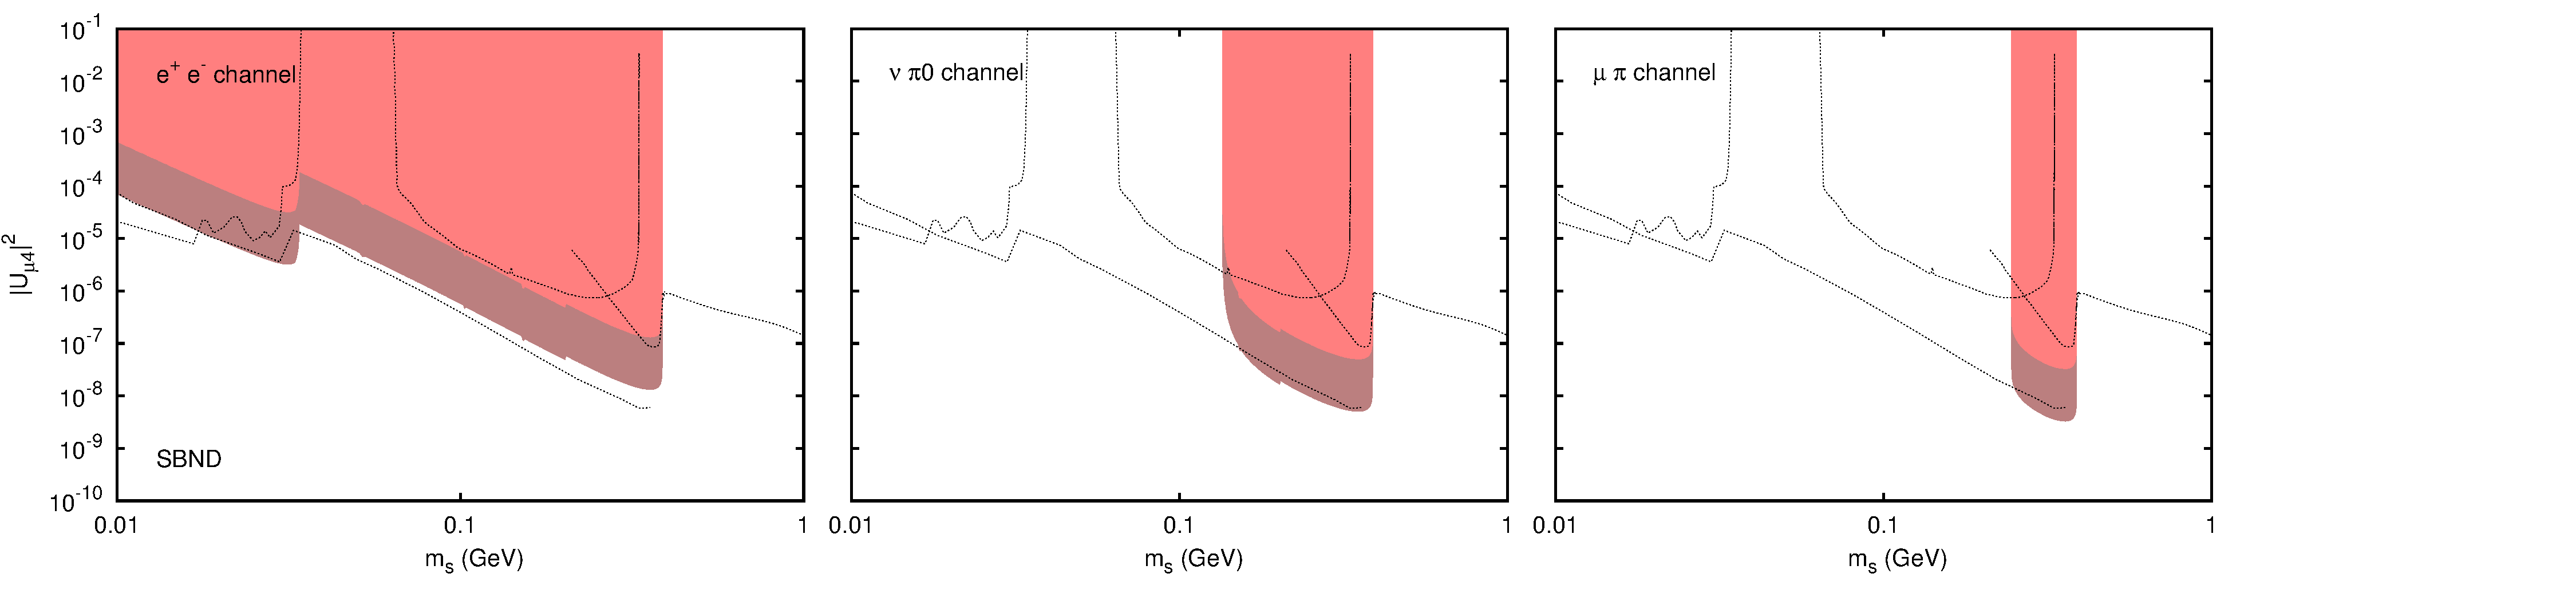
\includegraphics[width=1.0\textwidth,clip,trim=0 20 300 15]{figures/sbnd_all_panels_um4.pdf}
%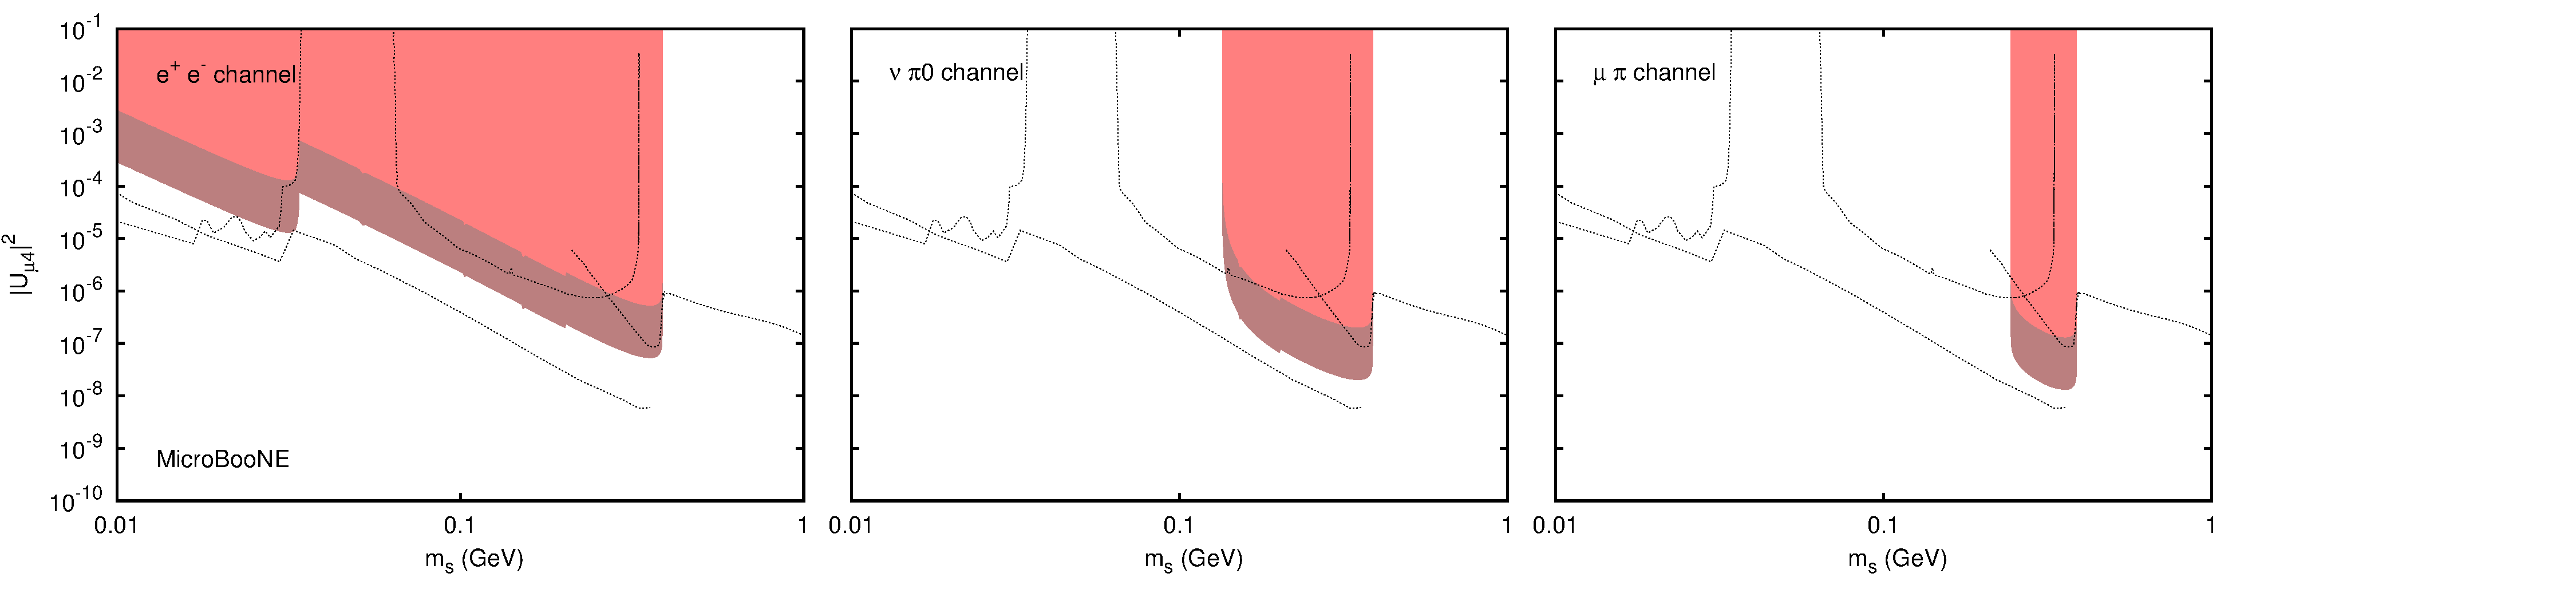
\includegraphics[width=1.0\textwidth,clip,trim=0 20 300 15]{figures/muboone_all_panels_um4.pdf}
%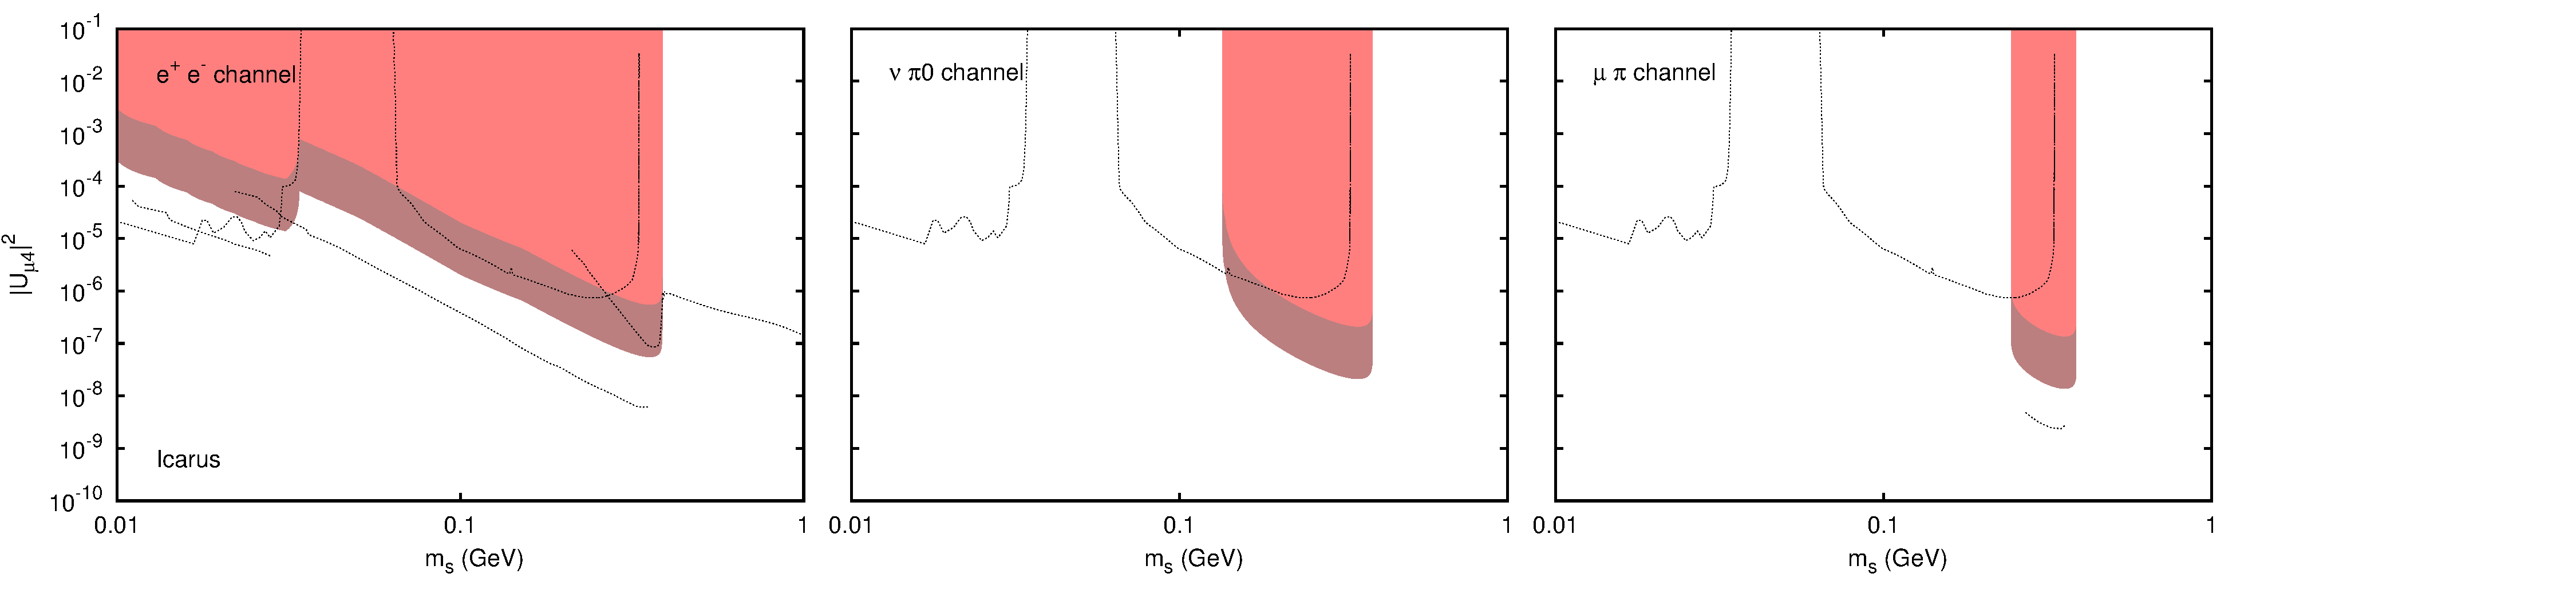
\includegraphics[width=1.0\textwidth,clip,trim=0 20 300 15]{figures/icarus_all_panels_um4.pdf}
%
%\caption{\label{fig:no_cuts_scaled_bkg_um4_only}The sensitivity contours based on the total
%number of events, assuming only mixing with the muon neutrino ( $\vert U_{e 4}\vert^2=\vert U_{\tau 4}\vert^2=0$), without cuts but with varying degrees of background
%suppression. We overlay the 95\% exclusion regions for $U^2$ and $m_s$ from
%previous experimental work.}
%
%\end{figure}
%


\section{\label{sec:baselineinterplay}Model comparison at the SBN complex}

%1. intro
Given the existing anomalies in short baseline neutrino experiments, including
MiniBooNE which operated in the Booster beamline, the possibility of seeing an
anomalous signature at the SBN complex should not be ignored. There are
competing theoretical explanations for existing excesses: oscillatory sterile
neutrinos \cite{Everyone...}, neutrino decay \cite{Pascoli, Schwetz}, neutrino
production and decay inside the detector \cite{Gninenko, Meloni, Us?}. Taking 
this as motivation, we consider here the differentiating characteristics of some 
different models of new physics in the neutrino sector. 

%2. features of SBN which are interesting
The combination of the three SBN detectors, all operating with the same
technology in the same neutrino beam, allows for distinctive signatures of new
physics. In this section, we assess the potential for SBN to investigate an
excess of events seen at one or all of the detectors. 
%
Secondly, we discuss the role of event timing information can
have on model selection.  Timing delays between excesses would be strong
evidence for heavy particles propagating between source and detector, and we
explore how the study of timing effects could be used to bound the mass of the
particle in a model independent fashion.

We consider three possible explanations for an anomalous excess of particles:

%3. models to be distinguished between
\subsection{Comparison between sterile neutrino oscillations and decays in flight}

The oscillatory sterile explanation of low-energy anomalies in neutrino data is
theoretically appealing if not entirely phenomenologically satisfactory. Either
way, the SBN complex will be able to place important constraints on these
models. With the purposes of our present study in mind, there is little chance
that an oscillatory sterile could be confused by a MeV scale decaying sterile.
The signal for an oscillatory sterile would be a single electron, arising from
a charged-current quasi-elastic processes. There are no channels available to a
decaying sterile neutrino which could produce such a signal without an
additional (charged) particle. 

\newtext{PB}{Would it be worth writing anything here about electron(s)/photon
discrimination?}

There is also a strong difference in the baseline dependence which may be
visible at SBN. \newtext{PB}{It feels a bit pointless to fill this section
out.}

\subsection{Differences between decays in flight and production/decay in situ}

The model of Gninenko \cite{Gninenko:2009ks,Gninenko:2010pr} which seeks to
explain the MiniBooNE excess through the production and decay of a new sterile
fermion inside the detector, has received significant attention in the
literature. This model general requires quite a large non-minimal transition
magnetic moment to ensure sufficient decays. 

Our model of decaying sterile neutrinos in flight is formally similar to the
Gninenko model, albeit with a more general set of observable final states. The
main difference lies in the region of parameter space for which a signal would
be generated for any beam dump experiment. With the high decay rates of
Gninenko, no significant sterile component would exist in the beam by the time
the particles reached SBND. Vice versa, the minimal sterile model simply does
not have a high enough decay rate to see any decays after particle productions
inside the detector via mixing-matrix element mediated neutral current
scattering. However, without a knowledge of the true parameter space, these two
models could be confused. The main way to distinguish them would be through
their spectrum of events. Although both models produce visible particles
through sterile neutrino decay in flight, the additional neutral current
cross-section required by the Gninenko-type sterile suppresses the lowest
energy events. As can be seen in \reffig{fig:XXX}, we see a marked difference
between these signals at SBND. If we factor in the cut-based analysis that was
performed in the preceeding section, we see that the model in this paper does
lose a significant number of events from the lowest bins. To separate these
events cleanly, the analysis should be optimised to keep as many of these
lowest energy events as possible. 

\newtext{PB}{A relevant point here would be the use of timing.}

%
%\subsection{Scaling behaviour of event rates}
%
%Any source of excess events which is induced by the neutrino beam should
%inherit a $L^{-2}$ dependence on baseline distance from the dispersion of the
%neutrino flux. Between three detectors, this would generate a distinctive
%relative enhancement of the signal at SBND and relative suppression of the
%signal at \icarus\ compared to a fixed nominal excess at \muboone. This is in
%contrast to, for example, an excess of misidentified cosmogenic events which
%would have no baseline dependence.
%
%New physics may cause a signficant dependence on baseline. One of the much
%discussed ways to explain an excess of events at a short baseline neutrino
%experiment is through sterile neutrino oscillations. The rates predicted at
%three different detectors depend crucially on the respective distances from
%source to detector according to the oscillation prbobability. In the scenarios
%discussed in this paper, we also see baseline dependence coming from
%\refeq{eq:prob}, albeit in a very different form. For most of the parameter
%space, we predict no significant baseline dependence on the event rates
%at the three detectors, once the $1/L^2$ dependence of the flux is removed;
%however, for large decay rates we see a baseline dependent effect. This is
%shown in \reffig{fig:baselineratios}, where the event numbers for $e^-e^-$
%decay are shown as ratios between the three detectors. These have been scaled
%to remove the baseline dependence of the flux.  The four lines for each
%detector show the 100\%, 75\%, 50\% and 25\% contours (where the further
%detector sees fewer events). Such decay rates are forbidden in the minimal
%extension of the SM incorporating MeV scale sterile neutrinos
%\newtext{PB}{True?}. In a non-minimal model, it remains possible that decays
%with decay lengths of the order $100$~m could exist, leading to a very 
%significant depletion of events at the further detectors.
%
%We show in \reffig{fig:baselineratios} a plot highlighting the contrasting
%behaviour between these alternative explanations for an excess seen at the SBN
%complex. In these plots we assume a fixed $100$ events at \muboone\ and observe
%the distribution of events at the other sites for different models of new
%physics.

\subsection{\label{sec:timing_physics}Timing for model discrimination}
In addition to being able to reduce beam-related backgrounds by studying the inter-bucket windows, the timing of the observed events can also be used to discriminate between different models, as well as give an independant measurement of the sterile mass.  
We can estimate the impact of this information on the model discrimination
given an knowledge of the precision in timing measurements of the sterile
neutrinos. Elementary special relativity tells us that for an arrival time delay (behind a luminal particle) over a distance $L$ denoted by $\Delta T$, the mass of a sterile neutrino with an energy $E$ can be reconstructed as 
%
%\[    \Delta T = \frac{L}{c}\left(\frac{E}{\sqrt{E^2-m_N^2}} - 1\right). \]
%
\[ m_N = E\sqrt{1-\frac{1}{\left(1+\frac{c\Delta T}{L}\right)^2}}. \]

To determine the prospects for measuring $m_N$ using this information we
have generated Monte Carlo event data tagging each event by an arrival time.
We account for a systematic uncertainty associated with the time measurement as
well as the energy reconstruction. We smear energy to represent detector effects as described above, and aditional smear the time of each event with a finite time resolution of $\sigma_T  \approx 1$ for SBND and ICARUS. As the absolute timing of the event is not known, only the relative timing since the last bucket, $\Delta T$, one can obtain up to 81 degenerate solutions for the sterile mass from any given event depending on the placement in the spill structure. By only studying the initial few buckets one can elleviate the problem, however, it also reduces the signal statistics by $\mathcal{O}$(0.01) and so this edge effect information is ignored in this analysis.
\newtext{MARK}{Working on this last plot for here, generated all the data just need to get an answer.}
\begin{figure}[t]
\center
\includegraphics[width=0.6\textwidth]{figures/timing_scatterplots.pdf}
\caption{\label{fig:tof_scatter} The distribution of events at ICARUS for a 150, 250 and 350 MeV sterile decaying to $e \pi$ in energy and timing delay from last beam bucket. High energy events can be used to distinguish the decaying sterile masses.}
\end{figure}


\section{Conclusions}

In this paper, we
have studied its capabilities of the Fermilab Short-Baseline neutrino facility to constrain decaying sterile neutrinos with
masses around the MeV scale. To make a fair assessment of the potential to
constrain these models, we have performed a simple cut-based analysis of the dominant
backgrounds and signals and shown that in conjunction with accurate timing measuremnts high levels of background suppression
can be expected resulting in close to backgroundless searches in all channels studied. Using these background estimates,
we have performed a sensitivity analysis to the parameters of the minimal
extension of the SM with a novel sterile neutrino. Despite having significntly lower statistics than the full SBN, we show $\mu$BooNE could be sensitive to such decays and any observation would correspond to a strong signal in both SBN and ICARUS when they later come online.  We have also motivated searches for non-minimal models, which in particular could lead to observable
decays over a wide range of parameter space which is conventionally excluded by
theoretical assumptions on the decay rates themselves. We argue that these
decay rates are actually \emph{unconstrained} in published work, and show that
the SBN could place the first direct bounds on these processes. 

\acknowledgments

We would like to thank Andrezj Szelc for his input to various elements of this
work, and also to Jonathan Asaadi for helpful discussions at the start of this
project.

This work has been supported by the European Research Council under ERC Grant
“NuMass” (FP7-IDEAS-ERC ENC-CG 617143) and by the European Union FP7
ITN-INVISIBLES (Marie Curie Actions, PITN-GA-2011-289442).

\appendix
\section{Potential Backgrounds\label{sec:bg}}
In order to estimate the effect of expected backgrounds on the sensitivity we have performed a Monte-Carlo analysis using the neutrino event generator GENIE (cite GENIE). This provides us with generator level information about the kinematics of the beam-driven backgrounds, with rates normalised off expected NC and CC inclusive values as published in the SBN proposal. Energy and angular smearing is then implemented to allow for approximate estimates of the effects of detector performance to the level necessary for this analysis, without the need for a full GEANT detector simulation. Energies are smeared according to a Gaussian distribution around their true MC energies, with a relative variance $\sigma_E/E = \xi/ \sqrt(E) $, where $\xi$ is a detector dependant resolution. For this study we take the energy resolution for EM showers, muons and protons to be 15\%, 6\% and a conservative 15\% respectively. We take the angular resolution of LAr to be $1^{\circ}$. 

Of utmost importance in all studied channels to distinguishing signal and background is the identification of a scattering vertex. Any hadronic activity localized at the beginning of the lepton track is a smoking gun signal for beam related scattering from deep-inelastic or quasi-elastic scattering. Therefore any event containing one or more reconstructed protons or additional hadrons is rejected outright. For counting this proton multiplicity we assume an detection threshold of 21 MeV on proton kinetic energy in liquid Argon, after smearing. Background events that contain less than this and events that do not contain any protons, such as events originating from coherent pion production, remain a viable background and further rejection must come from the kinematics of the final state particles only. 

All two body visible decays discussed below have a powerful discriminator in the reconstructed invariant mass of the charged particle pair, e.g  $M_{l^\pm \pi^\mp}^2=m_l^2+m_{p^\pm}^2+ 2(E_l E_\pi - |P_l||P_\pi|\cos\theta_\text{sep})$ for $\nu_N \rightarrow \pi^+ l^-$, which sum to that of the the parent sterile (within detector resolution), where as the background is expected form a broad spectra spanning the energies of incoming neutrino. Additionaly, two body decays allow for reconstruction of the parent sterile angle with respect to the beamline which is assumed to be close to on-axis, unlike the more isotropic backgrounds. We found $\approx 95$\% of reconstructed sterile from two bodys decays were below $4^\circ$ relative to the beamline and we cut all events greater than this.

\begin{figure}[h]
\center
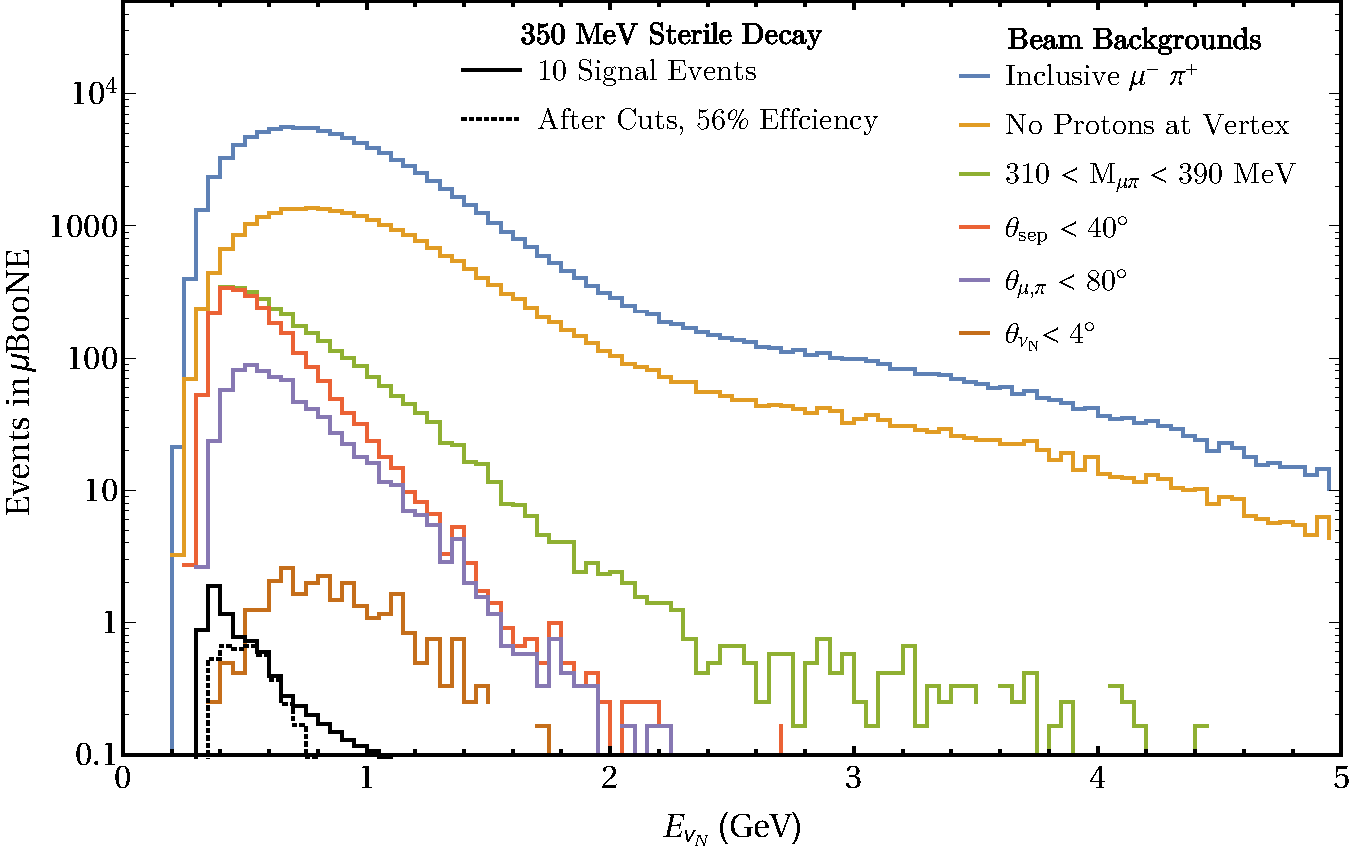
\includegraphics[width=0.6\textwidth,clip,trim=0 0 0 0]{figures/mu_pi_cutflow.pdf}
\caption{\label{fig:mu_pi_cutflow} Reconstructed sterile energy spectra for CC$\nu_\mu$ backgrounds in comparison to a 350 MeV decaying sterile at $\mu$BooNE, normalised to 10 signal events. Total expected background of 98,013 events is reduced to $\approx$ 27 by successive kinematic cuts utilising expected differences between decay and scattering behaviour. }

\end{figure}
\subsection{$\nu_N \rightarrow \mu^\pm \pi^\mp$ and $\nu_N \rightarrow e^\pm \pi^\mp$   }
The dominant backgrounds to the sterile decays we are interested in will be genuine $\pi$-lepton production associated with
the neutrino beam. So-called CC1$\pi^+$ events are defined as the associated production of a charged pion from the standard CC process which produces a lepton. These events can be produced incoherently, often with large hadronic activity, or from coherent scattering, where the neutrino scatters from the whole nucleus. These coherent interactions tend to produce more forward decay products and will be another significant source of backgrounds. Coherent cross-sections for these processes have been studied in MiniBooNE \cite{Wascko:2006tx}, \minerva \cite{Eberly:2014mra} and lately T2K and cross-sections appear to agree with Monte Carlo calculations based on the Rein-Sehgal model \cite{Rein:2006di, Rein:1982pf}.
Such a low $Q^2$ process tends to favour daughter pions and muons that are forward going, kinematically very similar to decays in flight, as well as no observable nuclear activity and as such are a potent background.\\ 

The expected numbers of $e \pi$ events in the SBN detectors is significantly smaller than that of the $\mu \pi$ channel, as the fraction of intrinsic $\nu_e$ in the BNB beam is of
$\mathcal{O}(1\%)$ level in comparison to $\nu_\mu$. However, there will also be additional backgrounds to the
$e \pi$ channel originating from the dominant $\nu_\mu$ beam. CC $\nu_\mu$ events which contain an additional photon $(\mu+\gamma)$, or 1 reconstructed photon from a $\pi^0$ decay, have the potential to be be mis-identified as an $(\pi
e)$ event, provided the muon has a sufficiently short track length, $<$ 0.5 m, in order to mimic a $\pi^-$. Additionally the photon must be mis-identified as an electron, with an efficiency of 94\%, and furthermore, must convert to an $e^+e^-$ pair close enough to the interaction vertex as so there is no visible gap. Thus we accept 6\% of all CC $\mu+\gamma$ events whose photon converts within 3cm, and whose muon track length is less than 0.5m. Combined with the rejection of events with any vertex activity, this reduces the number of background events to below that expected from intrinsic CC $\nu_e$ pion production. As energy resolution for EM showers is lower than muons, the invariant mass cut is less powerful requiring all events have an invariant mass below 500 MeV. 

Additional kinematic cuts are selected to further decrease backgrounds. A cut on lepton-pion opening angle, $\theta_{l \pi} < 40^\circ$ as well as indicidual emission angles, $\theta_{l,\pi} < 80^\circ$, reduces the potential background from 1,153,090 in SBND to approximately 323 events for $\mu^- \pi^+$.  \reffig{fig:mu_pi_cutflow} shows the background rejection capability of LAr as each additional cut is implemented in $\mu$BooNE, in comparason to a 350 MeV sterile decay. The $e^- \pi^+$ channel is one of the cleanest channel under consideration, with 9223 events in SBND reducing to 22 expected events post cuts, and with $\mu$BooNE and ICARUS expecting $\mathcal{O}(1)$ events from beam driven backgrounds.


\subsection{$\nu_N \rightarrow \nu_\alpha e^+ e^-$ and $\nu_N \rightarrow \gamma \nu_\alpha$ }
A sufficiently boosted, and thus overlapping, $e^+e^-$ pair is topologically indistinguishable from a converted photon in a LAr detector. Additional, non-topological measures such as the rate of energy loss, $dE/dx$, is also identical to a pair-converted photon. Thus we split this channel into two sub categories, when the $e^+e^-$ is overlapping and photon-like, defined to be all events whose angular separation is $\leq 3^\circ$\cite{Spitz:2011wba} and all remaining separable two track events. The opening angle between the $e^+e^-$ in a photon pair production scales roughly as $\approx m_e/E_\gamma$, with $3^\circ$ corresponding to 100 MeV and used as a lower bound on energy. These backgrounds are also applicable to the $\nu_N \rightarrow \nu_\gamma \nu_\alpha$ channel.\\ 

Any standard process producing a lone stray photon is thus a possible source of backgrounds for the photon-like $e^+e^-$ channel. The predominant source of this in all three SBN detectors is the decay of a neutral pion in which a single photon is not resolved or escapes the fiducial volume. This background, however, is relatively isotropic in distribution and of lower energy that the signal, in stark contrast to the very forward signal. Thus we apply a cut on visible photon energy, $E_\gamma \geq 300 $ MeV and angle of the observed photon to the beamline, $\theta_\gamma \leq 5^\circ$. In conjunction with the requirement that no vertex activity is recorded, this reduced the number of expected events from 42,580 to 176 events in SBND, while retaining a signal efficiency of 93\%.

For the opposite scenario both daughter electrons have a well defined, and large, separation and thus can cleanly be identified as two distinct single electron showers. There are no significant processes that produce high energy, distinguishable $e^+e^-$ pairs in a standrd neutrino beam.  Instead the majority of the backgrounds are due to misidentifying photons, which are abundant, as electrons. This can either be a single photon alongside a CC $e^-$ event or the more common NC $\pi^0$ production in which both of the underlying photons are mis-identified as electrons. As both of these backgrounds require the photons to mimic electrons originating from a single decay vertex, we also require that all photons pair convert within 3cm of the start of the electron track in the case of CC $\nu_e$ backgrounds, or both photons convert within 3cm of each other in the case of NC $\pi^0$ backgrounds. Further more, each event passing the above cuts is rejected with a 94\% efficiency using measurements of the rate of energy loss, $dE\/dx$. All remaining events are kept as backgrounds. To further reject backgrounds we apply a cut on angle of separation between the distinct $e^-e^-$ tracks of $\theta_\text{sep}\leq 40 ^\circ$ and total energy, $E_{e^+}+E_{e^-} \geq 100$ MeV. This reduces the number of expected backgrounds from 173 events to 5 events in SBND. 

%\begin{figure}[h]
%\center
%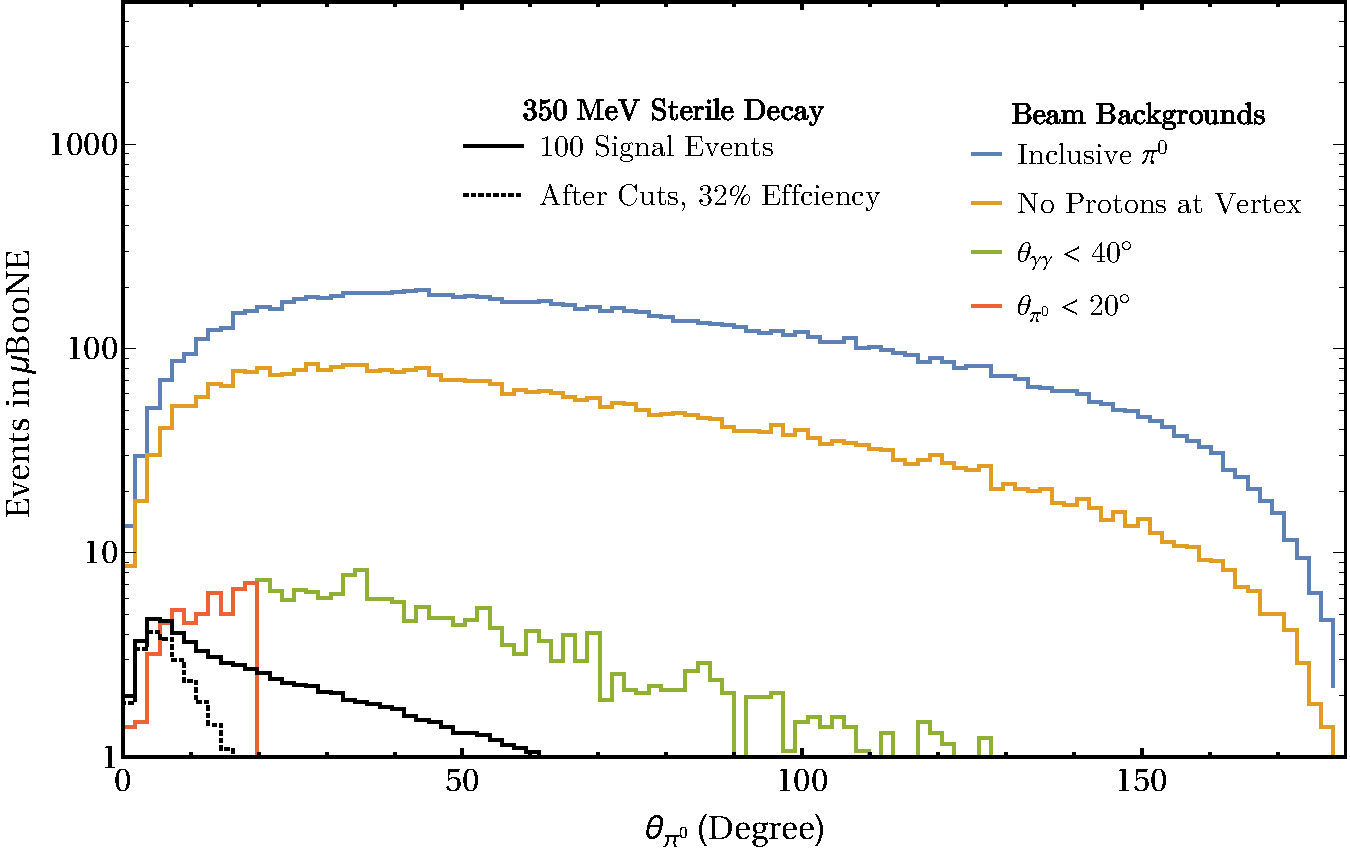
\includegraphics[width=0.6\textwidth,clip,trim=0 0 0 0]{figures/nu_pi0_cutflow.pdf}
%\caption{\label{fig:nu_pi0_cutflow} Reconstructed $\pi^0$ angular spectra with respect to the beamline for NC$\nu_\mu$ backgrounds in comparison to a 350 MeV decaying sterile $\nu_N \rightarrow \nu_\alpha \pi^0$ at $\mu$BooNE, normalised to 100 signal events. Total expected background of 10,813 events is reduced to $\approx$ 51 by utilising forwardness of pion produced in decays, alongside the requirement of no hadronic activity. }
%\end{figure}

\subsection{$\nu_N \rightarrow \pi^0 \nu_\alpha$}
Although a sub-dominant decay mode when steriles mix with electrons alone, when one considers non-zero $\vert U_{\mu4}\vert^2$ the branching ratio of $\nu_N \rightarrow \nu_\mu \pi^0$ becomes dominant for a mass window $\approx 140 \rightarrow 240$ MeV. There is no known experimental publication of $\nu_N \rightarrow \nu_\alpha \pi^0$ in the literature, mainly due to the large expected backgrounds. Single neutral pions are produced in great numbers at the three SBN facilities, so the lack of any nuclear recoil is crucial in eliminating the incoherent neutral pion production background. As the $\pi^0$ itself is not visible, we focus on the reconstructed pion energy and angle, inferred from measuring the resultant photons energy and angle, smeared as usual to model detector effects. Only events in which both photons convert inside the fiducial volume are accepted. SBND expects 127,211 $\pi^0$ events, of which $\approx 602$ survive all cuts with a signal efficiency of 32\% for a sample 350 MeV sterile. \\ 

To summerise, we collect the total numbers of beam-induced background events expected at the three SBN below in \reftab{tab:Rates}, both before and after we apply all visible vertex and kinematic cuts as described above. One can see that LAr provides an impressive level of background rejection, with \muboone and ICARUS being close to backgroundless in many channels, and SBND expecting only $\mathcal{O}(100)$ events in all channels.

\begin{table}[t]
\centering
\begin{tabular}{ l | l |  l | l |  }
	Signal Channel & Events @ SBND & \muboone\ & ICARUS \\
\hline\hline
$\mu^\pm \pi^\mp$ &  1,530,900  & 98,013 & 164,716\\
													  w/ Cuts &323 & 27 & 46 \\ \hline
$ e^\pm \pi^\mp$ &  9,228  & 784 & 1,317\\
													  w/ Cuts &22 & 2 & 3 \\ \hline
$ \nu_\alpha \pi^0$ &   127,217 & 10,813 & 18,172\\
													  w/ Cuts &603 & 51 & 86 \\ \hline
$ e^+e^- \text{ (Separate)} $ & 173 & 14 & 24\\
													  w/ Cuts &5 & 0.3 & 0.5\\ \hline
$ e^+ e^- \text{ or } \gamma \text{ (Photon-like)}$ &  42,580 & 3,620 & 6,082\\
													  w/ Cuts &176 & 46 & 110 \\ 
 \hline \hline

\end{tabular}
\caption{\label{tab:Rates} A summary of the main sources of backgrounds for each channel studied, before and after spectral and particle ID cuts are applied as discussed in section \ref{sec:bg}. }
\end{table}


\subsection{Non-Beam related backgrounds}
Cosmogenic backgrounds are expected to be significantly smaller in comparison to beam related backgrounds. In the case of cosmic muons, \icarus\ expects to see approximately $2.5 \times 10^{6}$ cosmic events in the 211 second beam spill,
and are reduced to approximately 5 events expected after utilizing the spill
structure, scintillation light patterns and cuts on $\frac{d E}{d x}$
\cite{Antonello:2015lea}.  Alongside this impressive cosmic rejection, our signal
events are focused heavily along the beamline, hence we do not expect cosmics
to be a major source of background to any channel. In situ beam-off cosmic studies will also allow potential backgrounds to be extremely well understood by the time of an analysis such as this, are so are not included in this analysis. 

\section{PS-191 Bound Repoduction}

As a consistency check of our methodology we reproduce here the bounds on $|U_{e4}|$ and $|U_{\mu 4}|$ for sterile masses below $m_\pi$ as published by PS-191. The detector geometry is assumed to be
$6\text{m} \times 3\text{m} \times 12 \text{m}$ and was located 128m downstream
of the Beryllium target using 19.2 GeV protons from the PS proton beam.  Fluxes
of all neutrinos produced from pion sources at PS-191 were obtained from
\cite{ps191THesis}. No accurate kaon sources could be obtained and as such only
low mass bounds are reproduced here. It must be noted that PS-191 ignored all
neutral current contributions to $\nu_N \rightarrow \nu_\alpha e^+ e^-$ and
assumed the sterile neutrinos were Dirac particles; the effect of this is
that the bounds published are not directly comparable to the minimal model discussed
above, and must be scaled appropiately. The bounds reproduced are in good agreement with published data.

\begin{figure}
			  \centering
			 
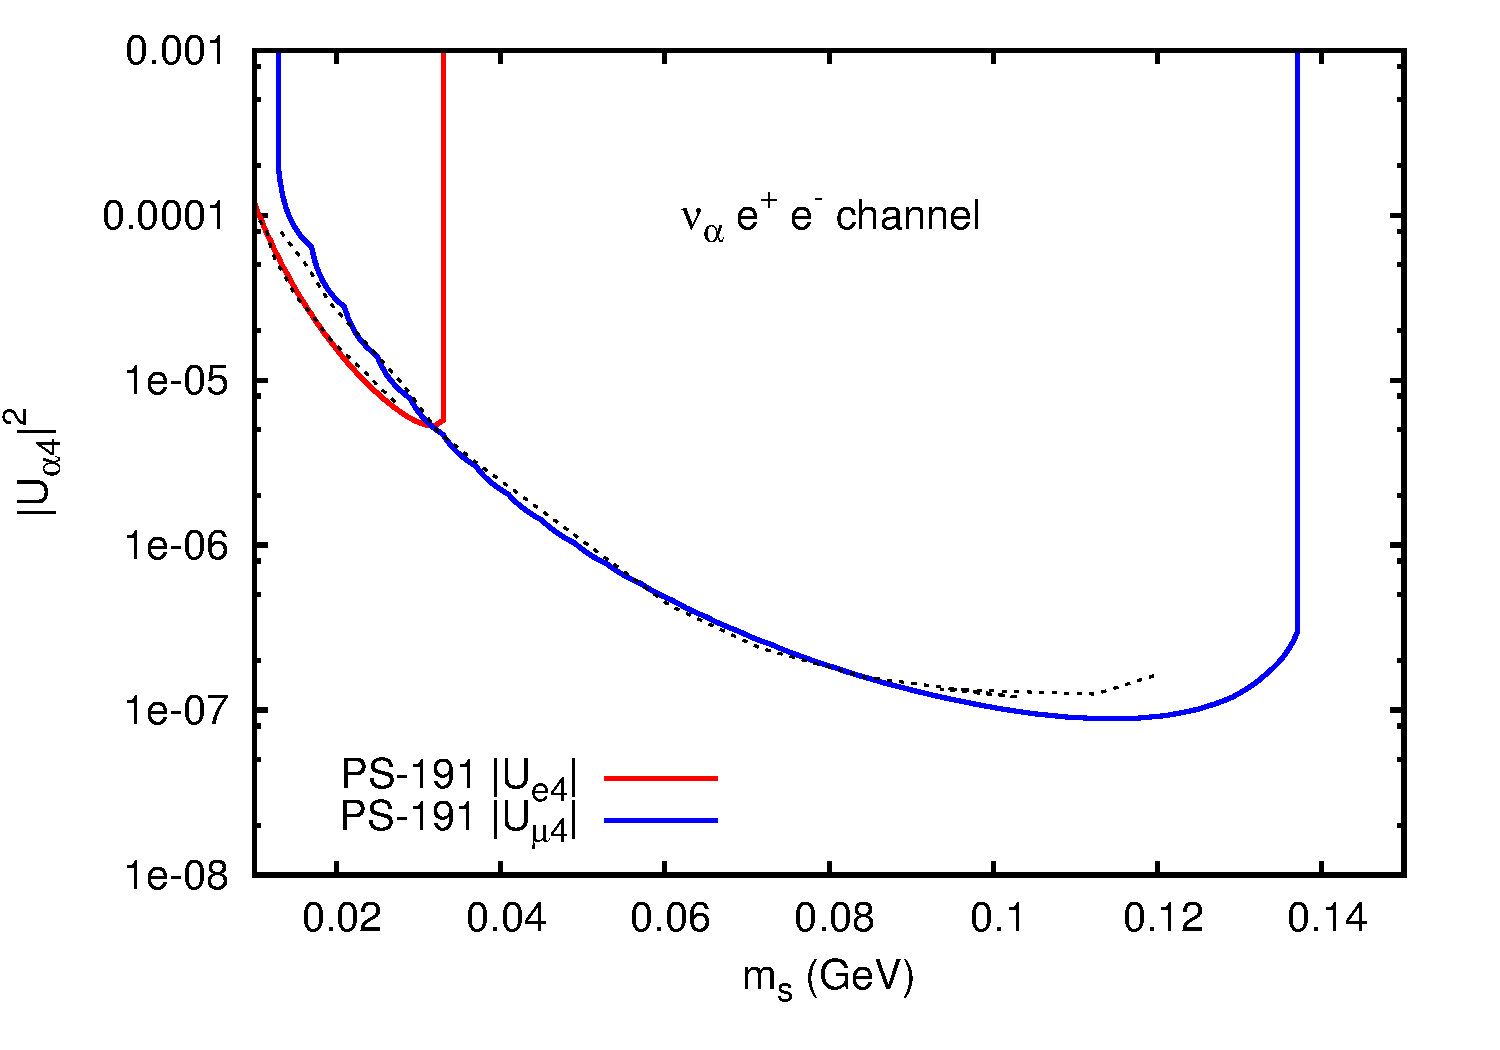
\includegraphics[width=0.5\textwidth]{figures/PS-191_test.pdf}
\caption{\label{fig:ps191test} Estimated bounds on $|U_{e4}|^2$ and $|U_{\mu 4}|^2$ for a Dirac heavy sterile neutrino decaying to $\nu_\alpha e^+ e^-$ at PS-191. The dotted black lines are the 90\% C.L results as published by PS-191, and the blue and red curves are the results of our simulation for $0.86 \times 10^{19}$ POT.}
\end{figure}


\section{To do list}

\begin{enumerate}


\item Decide what statistical method to use? Do we do a spectral fit?

\item How does eventrate actually deal with spectra things? Can we modify it to 
do spectral plots or even fits?


\item \newtext{MARK}{Working on} Generagte efficiency file from above cuts.

\item \newtext{MARK}{Working on} Use the efficiency files from previous point to produce new plots of
sensitivity.

\item Implement $\nu\gamma$ decay rate. 

\item Compute plots for enhanced decay rates to unobserved channels. Check that
the enhanced $\Gamma$ code works.

\item Do a bit more checking that the `unobserved' channels are indeed unobserved.

\item Baseline dependence + event timing = physics? (Decide what we can do with
event ratios + scaling, or timing analysis).  \emph{e.g.} see figure
\ref{fig:baseline_comp}.

\item \newtext{MARK}{Converted to timing.cxx to integrate into the new inflight observabes that contains smearing} Timing scatterplots to distingush sterile masses, currently two mathematica notebooks with scatterplot and nautilus plot calculations on DropBox (not gitable).

\item Turn on $U_{\tau 4}$,$U_{\mu 4}$ and $U_{e4}$ simultaneously. Think of
how we can push the analysis beyond the obvious by using flavour effects. Also
look at ratios of channels and ratios of events to see if we can get any
(broken) degeneracies that could actually be interesting \emph{i.e} SNO style
complementary measurements.

\item Keep refining text. Add introduction; write sterile decay section; structure 
the simulation details section; write conclusions etc.

\item \newtext{MARK}{Working on} Make nice version of branching ratio plot. Need to make prettier. \sout{Also, we probably need to cut it off at 
	$M_N\lesssim 500$ MeV, there are other decays allowed between 0.5 and 1 GeV (with $\eta$ and $\rho$)}.

\item \newtext{MARK}{Working on} Think if there's a nice plot showing the sterile effect on our fluxes.

%\item Actually compute a $95\%$ CL exclusion region for a fair comparison with
%bounds. \newtext{PB}{See comment directly below. (This isn't a total
%solution... but I spent a while reading about how to do this properly and I
%think it's pretty defensible. Perhaps more so than what we would do with
%log-likelihood ratios...)}.
%
%\item \sout{The $S/\sqrt{B} =1$ criterion is (if it's defensible at all) really a
%$1\sigma$ significance measure. I think we should at least switch it to
%$S/\sqrt{B} =2$ which is $2\sigma\approx 95\%$ in the Gaussian limit.}
%\newtext{PB}{I have done this and updated the plotting scripts.}


	\end{enumerate}

%\begin{figure}[t]
%\center
%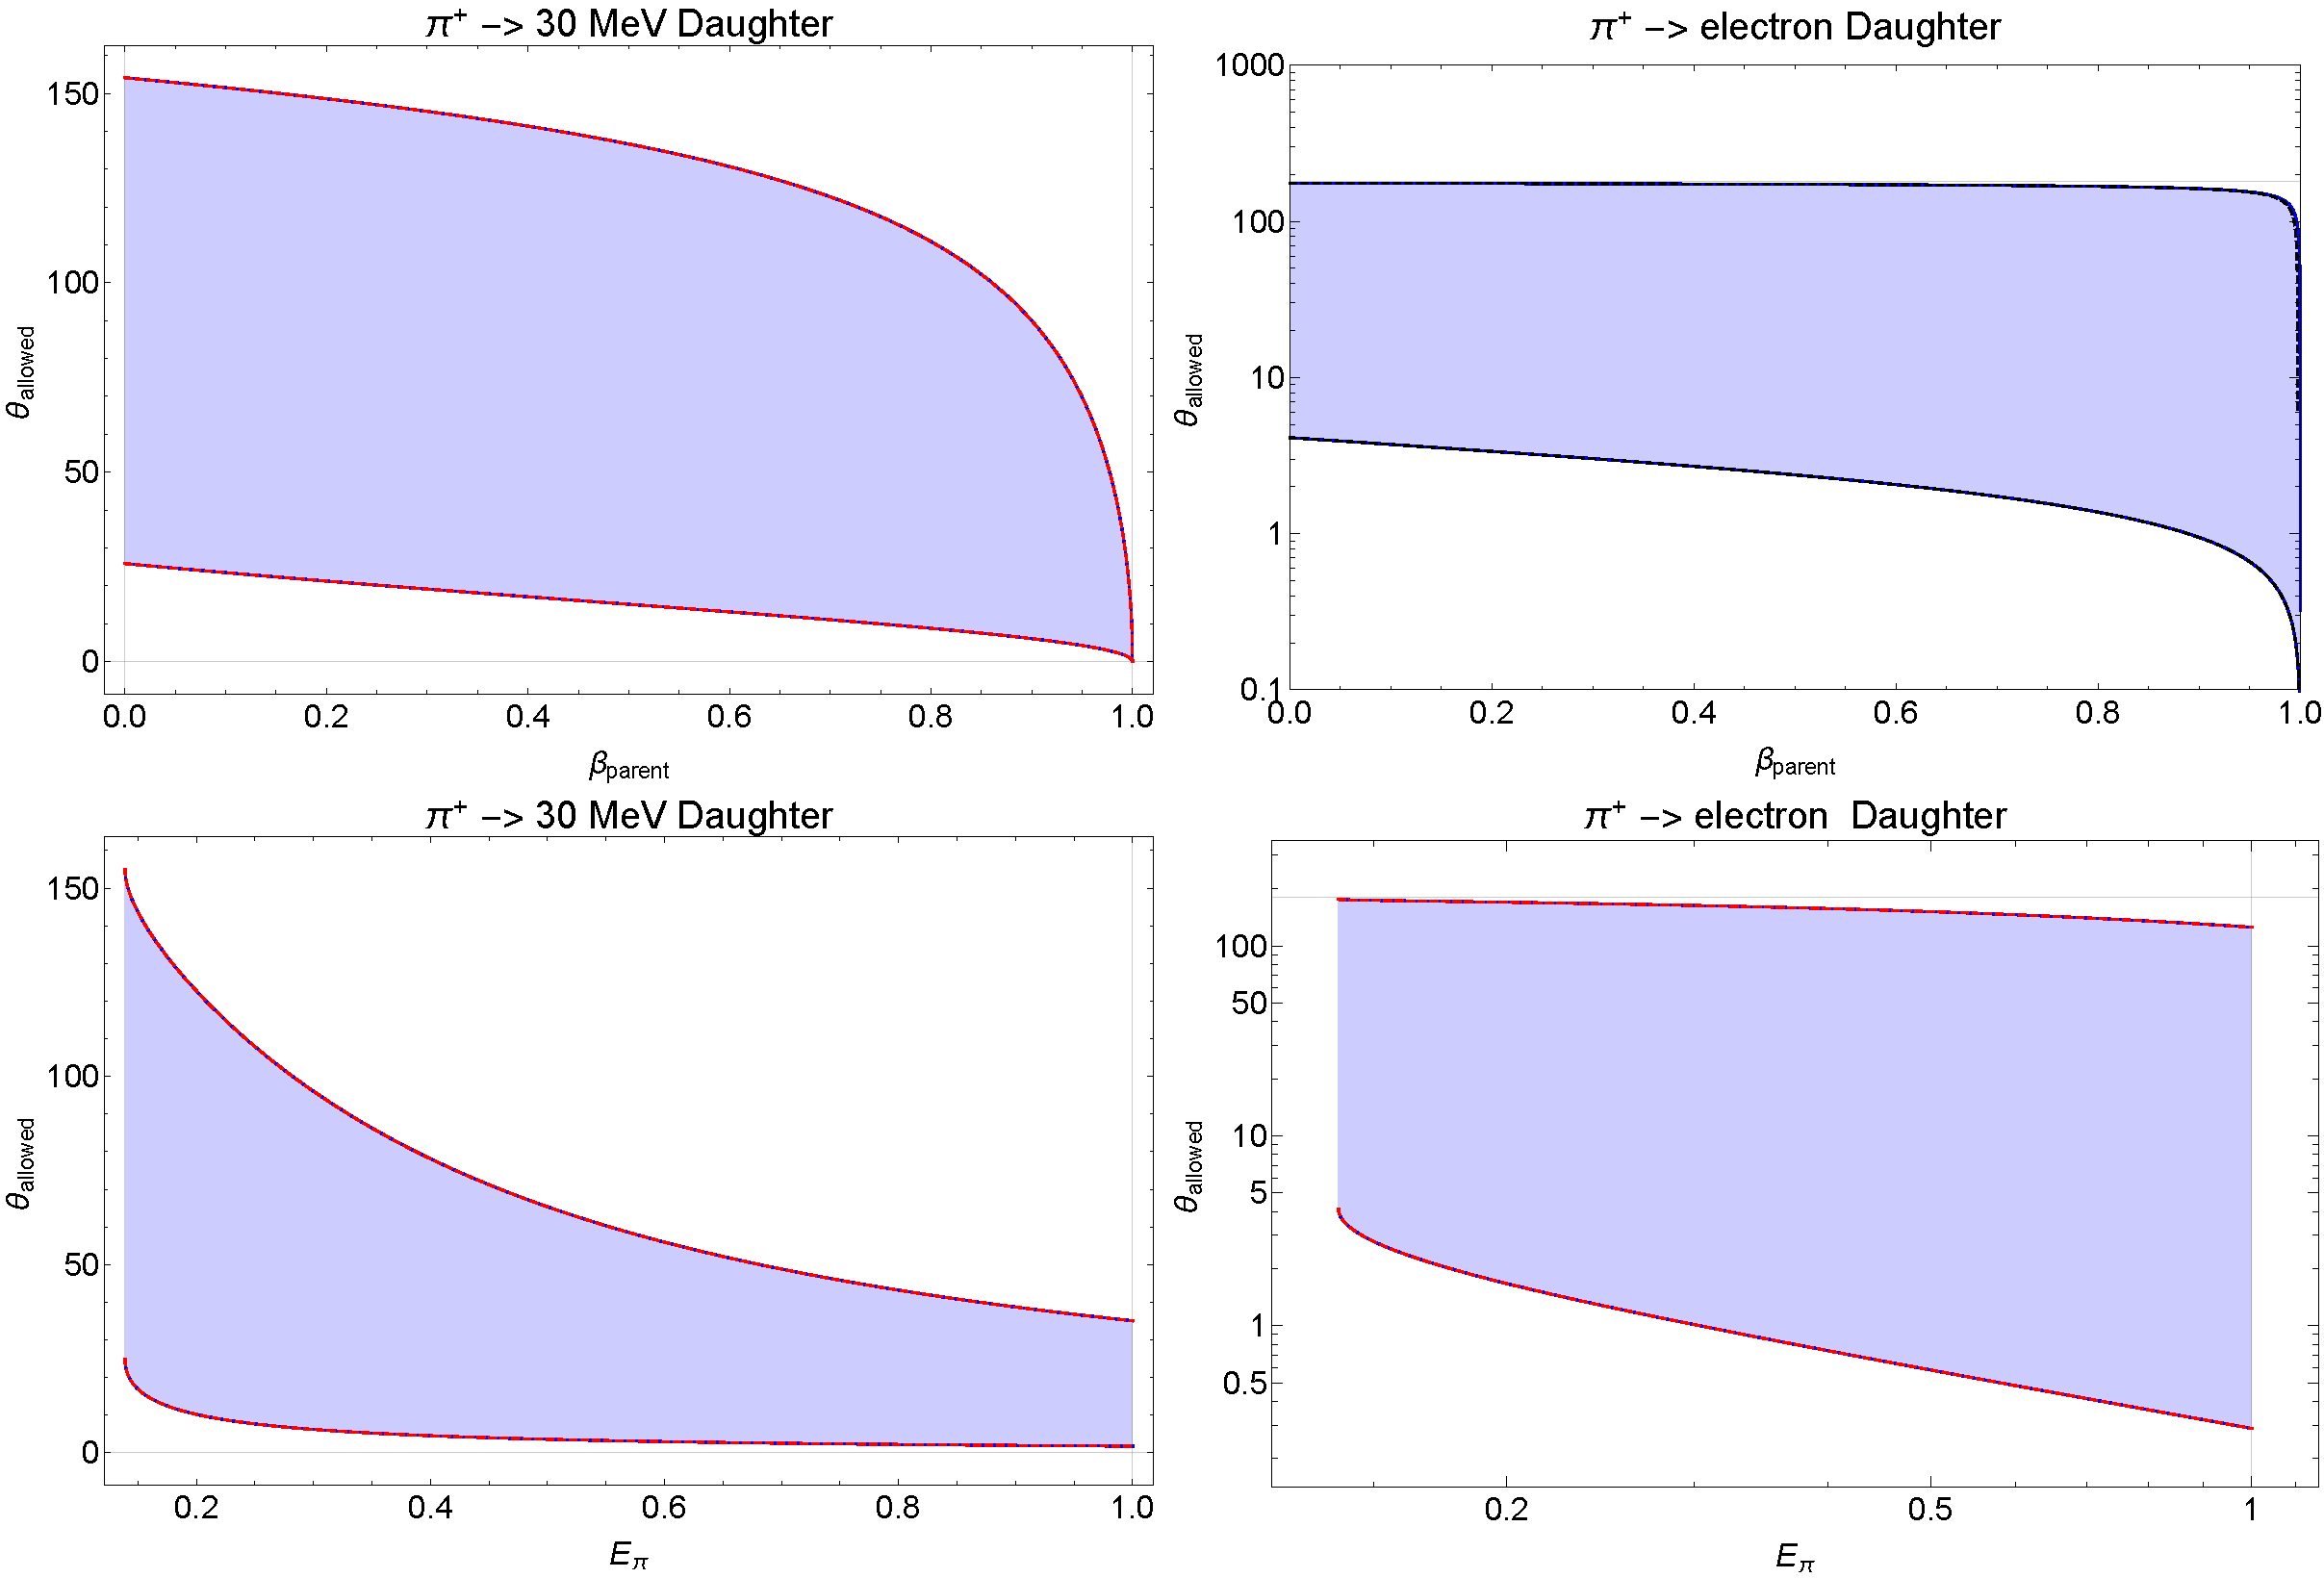
\includegraphics[width=1.0\textwidth]{figures/angles_boost.pdf}
%\caption{\label{fig:boost} Allowed angles in the decay $m_\pi \rightarrow a+b$ for $m_a 30$ MeV and $m_a=m_e$. In the limit of $m_a \rightarrow 0$ the entire $\beta_\pi - \theta_a$ plane is covered, which is pretty much what we were calculating today!   .}
%\end{figure}




%%%%%%%%%%%%%%%%%%%%%%%%%%%%%%%%
%%%%%%%%%%%%%%%%%%%%%%%%%%%%%%%%
%%%%%%%%%%%%%%%%%%%%%%%%%%%%%%%%

\bibliographystyle{apsrev4-1}
\bibliography{lib}{}

\end{document}

